% import gaya yang sudah disiapkan
\documentclass{gaya}

% import berbagai variabel
\titleind{Evaluasi Performa Arsitektur Fully Convolutional Networks untuk Segmentasi Mikrovaskular pada WSI Jaringan Ginjal Manusia: U-net dengan Modifikasi attention module} % yang ini untuk di cover
\titleindinline{Evaluasi Performa Arsitektur Fully Convolutional Networks untuk Segmentasi Mikrovaskular pada WSI Jaringan Ginjal Manusia: U-net dengan Modifikasi attention module} % yang ini untuk di dalam paragraf
\titleen{Evaluasi Performa Arsitektur Fully Convolutional Networks untuk Segmentasi Mikrovaskular pada WSI Jaringan Ginjal Manusia: U-net dengan Modifikasi attention module}

\fullname{Junpito Salim} % diisi nama Anda
\newcommand{\fullnamenc}{Junpito Salim} % diisi nama Anda
\idnum{120450086} % diisi NIM Anda

\approvaldate{-- Bulan 2024} % diisi tanggal penulisan
\newcommand{\approvaldatenc}{-- Bulan 2024}

\degre{Sarjana Sains Data}
\yearsubmit{2024} % diisi tahun penulisan
\program{Sains Data} % prodi
\dept{Sains} % fakultas

\firstsupervisor{Christyan Tamaro Nadeak, M.Si} % nama pembimbing 1
\nipnrkfirst{NRK } % diisi NIP atau NRK
\firstnip{1993120420211415}

\secondsupervisor{nama pembimbing 2, S.Si., M.Si.} % nama pembimbing 2
\nipnrksecond{NRK }
\secondnip{199008172020031003}

\headofdepartment{Tirta Setiawan,S.Pd., M.Si.} % nama koordinator prodi
\nipnrkhead{NIP }
\headnip{199008222022031003}

\def\tahapan{sempro} % opsi: sempro, semhas, sidang, atau final

%-----------------------------------------------
% Input tahapan Tugas akhir Anda saat ini
%-----------------------------------------------
% diisi dengan:
% sempro (jika dibuat untuk seminar proposal),
% semhas (jika untuk seminar hasil),
% sidang (untuk sidang), atau
% final (jika sudah final dan siap cetak)

\def\sempro{sempro}
\def\semhas{semhas}
\def\sidang{sidang}
\def\final{final}

\ifx\tahapan\sempro
\textta{Proposal Skripsi}
\textoncover{Diajukan sebagai syarat maju seminar proposal}
\textonapproval{Naskah Proposal Tugas Akhir } \else
\ifx\tahapan\semhas
\textta{Naskah Skripsi}
\textoncover{Diajukan sebagai syarat maju seminar hasil}
\textonapproval{Naskah Tugas Akhir untuk Seminar Hasil } \else
\ifx\tahapan\sidang
\textta{Naskah Skripsi}
\textoncover{Diajukan sebagai syarat maju sidang tugas akhir}
\textonapproval{Naskah Skripsi untuk Sidang Akhir } \else
\ifx\tahapan\final
\textta{Tugas Akhir}
\textoncover{Diajukan sebagai syarat untuk memperoleh gelar Sarjana}
\textonapproval{Tugas Akhir Sarjana } \else
\textta{SALAH INPUT!!!}
\textoncover{SALAH INPUT!!!}
\textonaproval{SALAH INPUT!!!}
\fi
\fi
\fi
\fi


% pemenggalan kata
% Hyphenation untuk Indonesia 
% @author  Ridlo Wahyudi Wibowo (+Kikun)
% 
% Tambahkan cara pemenggalan kata-kata yang salah dipenggal secara otomatis 
% oleh LaTeX. Jika kata tersebut dapat dipenggal dengan benar, maka tidak 
% perlu ditambahkan dalam berkas ini. Tanda pemenggalan kata menggunakan 
% tanda '-'; contoh:
% menarik
%   --> pemenggalan: me-na-rik
%
% selalu baca ulang dokumen untuk menemukan pemenggalan yang kurang tepat setelah pemenggalan 
% lain diperbaiki
\hyphenation{
    %spesial
    % alphabhet A
    a-na-li-sa
    a-tur 
    a-pli-ka-si 
    at-mos-fer
    ak-si
    ada-lah
    arc-se-cond
    % alphabhet B
    bumi
    ba-ngun-an 
    be-be-ra-pa 
    ber-in-ter-ak-si
    be-ru-pa
    be-ra-gam
    ber-ge-rak
    ber-ke-lan-jut-an 
    ber-pe-nga-ruh 
    ber-dasar-kan
    % alphabhet C
    ca-ri
    count
    cit-ra
    % alphabhet D
    di-sim-pan di-pim-pin de-ngan da-e-rah di-ba-ngun da-pat di-nya-ta-kan 
    di-sim-bol-kan di-pi-lih di-li-hat de-fi-ni-si
    di-ban-ding-kan
    di-si-mu-la-si-kan
    di-li-bat-kan
    di-se-bab-kan
    di-la-ku-kan
    di-je-las-kan
    di-tambah-kan
    di-temu-kan
    di-masuk-kan
    di-gu-na-kan
    di-ka-te-go-ri-kan
    di-ber-da-ya-kan
    di-a-frag-ma
    di-ha-sil-kan
    di-trans-for-ma-si
    di-bu-tuh-kan
    di-uta-ma-kan
    % alphabhet E
    e-ner-gi eks-klu-sif
    error
    equa-tor
    % alphabhet F
    fa-si-li-tas
    fitting
    fo-to-me-tri
    front-side
    for-mat-kan
    % alphabhet G
    ga-bung-an ge-rak
    % alphabhet H
    ha-lang-an
    % alphabhet I
    im-age
%    institut
    % alphabhet J
    % alphabhet K
    ke-hi-lang-an
	ke-sta-bil-an
    ku-ning 
    kua-li-tas ka-me-ra 
    ke-mung-kin-an 
    ke-se-pa-ham-an
    ko-e-fi-si-en
    kupang
    ko-or-di-nat
    % alphabhet L
    LINEAR
    ling-kung-an
    % alphabhet M
    mat-riks
    me-neng-ah
    meng-a-tas-i me-mung-kin-kan me-nge-na-i me-ngi-rim-kan 
    meng-u-bah meng-a-dap-ta-si me-nya-ta-kan mo-di-fi-ka-si
    meng-a-tur
    meng-gu-na-kan
		meng-ha-sil-kan
		me-nam-bah-kan
		me-nen-tu-kan
    me-nun-juk-kan
    meng-hu-bung-kan
    mem-per-li-hat-kan		
    me-man-fa-at-kan
    men-je-las-kan
    me-nye-bab-kan
    me-ru-pa-kan
    me-li-bat-kan
    meng-a-ki-bat-kan
    mengajari
    mengelilingi
    me-ning-kat-kan
    mem-be-ri-kan
    mul-ti-vari-ate
    me-mub-li-ka-si-kan
    % alphabhet N
    nya-ta non-eks-klu-sif
    ni-lai-nya
    non-eks-klu-sif
    % alphabhet O
    neo-wise
    ob-ser-va-to-ri-um
    ob-ser-va-tions
    % alphabhet P
    pack-age
    pro-grade
	pe-nye-rap-an 
	pe-ngon-trol
    pe-mo-del-an
    pe-ran  pe-ran-an-nya
    pem-ba-ngun-an 
    pre-si-den 
    pe-me-rin-tah 
    prio-ri-tas 
    peng-am-bil-an
    pen-di-di-kan
    peng-ga-bung-an
    pe-nga-was-an 
    pe-ngem-bang-an 
    pe-nga-ruh 
    pa-ra-lel-is-me 
    pe-rin-tah
    per-hi-tung-an 
    per-ma-sa-lah-an 
    pen-ca-ri-an 
    peng-struk-tur-an
    per-ban-ding-an
    per-kuliah-an
    pub-li-ka-si
    pe-nga-ta-log-an
    pe-nu-lis
    pen-cip-ta
    po-si-tion-ing
    pub-lish-ing
    pub-li-ca-tions
    % alphabhet Q
    % alphabhet R
    range
    ran-cang-an
    re-tro-grade
    % alphabhet S
    si-mu-la-si sa-ngat sur-vey sur-vei
    se-dang-kan
    stag-nan
    stan-dar-di-sa-si
	sub-sti-tu-si
    sub-bab
    sains
    skrip-si
    spec-tro-pho-to-me-tric
    sci-ence
    soft-ware
    % alphabhet T
    te-ngah
    ter-da-pat
    tisserand
	tri-angu-lar
    trans-for-ma-si
    Tilong
    terbuka
    % alphabhet U
    % alphabhet V
    % alphabhet W
    with
    % alphabhet X
    % alphabhet Y
    % alphabhet Z
    % special
    % < 3 huruf dan 1 huruf penggalan
    itu ini aku kau di si ke bui ibu tua tai tau ras pos ban dan cat cap cek cor akan alam asam ikan iring orang oli ubah ulang udang arang api elang amin aman iba 
    % asing
    log-book
}

% Isi keseluruhan dokumen
\begin{document}

% Sampul luar bahasa indonesia
\cover
\newpage

% Nomor halaman pembuka dimulai dari sini
\pagenumbering{roman}

% Sampul dalam bahasa indonesia
\coverdalam
\newpage

% Halaman pengesahan
\approvalpage
\cleardoublepage

% Halaman orisinalitas
\originalitypage
\cleardoublepage

% Halaman publikasi
\publicationpage
\cleardoublepage

% Abstrak Bahasa Indonesia
\begin{abstractind}
\justifying

\noindent Struktur mikrovaskular dalam ginjal manusia memainkan peran penting dalam fungsi tubuh, namun segmentasi secara manual memerlukan waktu yang lama dan keahlian khusus dalam histologi. Kompleksitas struktur mikrovaskular menjadi tantangan utama dalam pengembangan metode segmentasi otomatis pada citra histologi.. Penelitian ini mengevaluasi model Attention U-Net untuk segmentasi mikrovaskular pada Whole Slide Image (WSI) jaringan ginjal manusia dengan penambahan modul attention gate pada arsitektur U-Net guna meningkatkan akurasi. Dataset yang digunakan berasal dari Human BioMolecular Atlas Program (HuBMAP) dan telah dianotasi oleh ahli histologi. Model dilatih menggunakan optimizer Adam dengan batch size 4 untuk mencapai performa terbaik, kemudian dievaluasi menggunakan metrik Dice Similarity Coefficient (DSC), Intersection over Union (IoU), precision, dan recall. Hasil penelitian menunjukkan bahwa Attention U-Net unggul dibandingkan U-Net standar pada seluruh metriks utama. Mekanisme attention gate membantu model memfokuskan pada area relevan, sehingga meningkatkan kemampuan model dalam deteksi pembuluh darah kecil.

\bigskip
\noindent
\textbf{Kata kunci:} \textit{Attention U-net, Deep Learning, Dice Similarity Coefficient (DSC), Intersection over Union (IoU), Segmentasi Mikrovaskular}  % masukkan keyword
\end{abstractind}

\cleardoublepage

% Abstrak Bahasa Inggris
\begin{abstracteng}
\justifying
\emph{
The microvascular structure in human kidneys plays a crucial role in bodily functions, yet manual segmentation is time-consuming and requires specialized expertise in histology. The complexity of microvascular structures presents significant challenges in developing automated segmentation methods. This study evaluates the Attention U-Net model for microvascular segmentation in Whole Slide Images (WSI) of human kidney tissue by incorporating attention gate modules into the U-Net architecture to improve accuracy. The dataset used in this study was obtained from the Human BioMolecular Atlas Program (HuBMAP) and annotated by histology experts. The model was trained using the Adam optimizer with a batch size of 4 to achieve optimal performance and evaluated using metrics such as Dice Similarity Coefficient (DSC), Intersection over Union (IoU), precision, and recall. The results indicate that the Attention U-Net outperforms the standard U-Net across all key metrics. The attention gate mechanism enables the model to focus on relevant areas, thereby enhancing its capability in detecting small blood vessels.}
%%pada abstrak bahasa Inggris, separator desimal titik

\bigskip
\noindent
\textbf{\emph{Keywords :}} \emph{Attention U-Net, deep learning, Dice Similarity Coefficient (DSC), Intersection over Union (IoU), microvascular segmentation}
\end{abstracteng}

\cleardoublepage

% Motto
\motto
\begin{centering}
\vfill
\emph{We tune, we wait, and we trust the curve. Blooming, like convergence, unfolds in silence—never rushed, never late.\\[.6cm]}
\vfill
\end{centering}

\cleardoublepage

% Persembahan
\acknowledgment
\begin{centering}
\vfill
\emph{Untuk Emak dan Bapak\\di kampung\\[.5cm]}
\vfill
\end{centering}

\cleardoublepage

% Kata pengantar
%-----------------------------------------------------------------
%Di sini awal masukan untuk Prakata
%-----------------------------------------------------------------
\preface
\justifying
\noindent Puji syukur penulis panjatkan ke hadirat Allah SWT atas limpahan rahmat dan karunia-Nya, sehingga penulis dapat menyelesaikan skripsi ini dengan baik. Skripsi ini disusun sebagai salah satu syarat untuk memperoleh gelar Sarjana pada Program Studi Sains Data, Institut Teknologi Sumatera. Dalam proses penyusunan skripsi ini, penulis menerima banyak dukungan, bimbingan, dan bantuan dari berbagai pihak. Oleh karena itu, dengan penuh rasa hormat dan kerendahan hati, penulis menyampaikan ucapan terima kasih yang sebesar-besarnya kepada:

\begin{enumerate}
\item Bapak Tirta Setiawan, S.Pd., M.Si. selaku Koordinator Program Studi Sains Data Institut Teknologi Sumatera,
\item Bapak Christyan Tamaro Nadeak, M.Si. selaku dosen pembimbing pertama, atas bimbingan, arahan, dan motivasi yang berharga selama proses penelitian ini,
\item Ibu Luluk Muthoharoh, M.Si. selaku dosen pembimbing kedua, atas kesabaran dan dukungan yang senantiasa diberikan,
\item Ibu Dalima dan Bapak Syaiun, yang telah memberikan doa yang tiada henti, kasih sayang yang tak ternilai, serta dukungan moral dan material dalam setiap langkah penulis,
\item Teman-teman seperjuangan di kontrakan Tidurlah, atas canda tawa dan semangat selama masa studi,
\item Rekan-rekan dari Program Studi Sains Data angkatan 2020, yang telah menjadi bagian penting dalam perjalanan akademik ini. 
\end{enumerate}

Penulis menyadari bahwa penyusunan Skripsi ini jauh dari sempurna.
Akhir kata penulis mohon maaf yang sebesar-besarnya apabila ada kekeliruan di dalam penulisan skripsi ini.


\vspace{0.5cm}

\begin{flushright}
\begin{tabular}{p{7.5cm}l}
&Lampung Selatan, \approvaldatenc \\[2.5cm]
&\textbf{\fullnamenc}
\end{tabular}
\end{flushright}

\cleardoublepage

% Daftar Isi
\newpage
\addcontentsline{toc}{chapter}{DAFTAR ISI}
\tableofcontents

% Daftar Gambar
\newpage
\addcontentsline{toc}{chapter}{DAFTAR GAMBAR}
\listoffigures

% Daftar Tabel
\newpage
\addcontentsline{toc}{chapter}{DAFTAR TABEL}
\listoftables

% Daftar Singkatan
%\singkatan

\begin{flushleft}\vspace{0.5cm}
\begin{tabular}{p{1.5cm}p{2pt}l}
\textbf{A}\\
ADU & & Analog to Digital Units\\

\vspace{0.1cm}

\textbf{B}\\
BBU & & Belahan Bumi Utara\\
\vspace{0.1cm}

\textbf{C}\\
CCD & & Charge-Coupled Device\\
\vspace{0.1cm}

\textbf{M}\\
MPSAS & & Magnitude per Square Arcsecond\\
\vspace{0.1cm}

\textbf{N}\\
NOAO & & National Optical Astronomy Observatories\\
\vspace{0.1cm}


\end{tabular}
\end{flushleft}


% Daftar Simbol
%\simbol

\begin{flushleft}\vspace{0.5cm}
\begin{tabular}{p{.5cm}p{2pt}l}
     $m_x$ &  & Magnitudo\\
     $F_x$ &  & Fluks\\
     $\phi_x$ & & Tegangan pada \emph{clock cycle} CCD\\
     $k$ & & Ekstingsi\\
     $\epsilon$ & & Koefisien transformasi magnitudo $v$ ke $V$ \\


\end{tabular}
\end{flushleft}


\newpage

% Nomor halaman isi dimulai dari sini
\pagenumbering{arabic}

% Bab 1 pendahuluan
\chapter{PENDAHULUAN}
\section{Latar Belakang}
\label{section:latarbelakang}
\noindent Ginjal, organ vital dalam tubuh manusia, memiliki jaringan pembuluh darah kecil yang dikenal sebagai struktur mikrovaskular. Jaringan ini, dengan diameter kurang dari 100 mikrometer, memainkan peran penting dalam berbagai fungsi ginjal, seperti penyaringan darah, pengaturan tekanan darah, dan pengaturan keseimbangan elektrolit \cite{hu_multi-scale_2023}. Pemetaan struktur mikrovaskular secara detail menjadi kunci untuk memahami bagaimana sel-sel ginjal berinteraksi satu sama lain dan untuk mempelajari berbagai penyakit ginjal.
Upaya pemetaan sel-sel manusia secara komprehensif sedang dilakukan oleh Human Cell Atlas (HCA) dari Chan Zuckerberg Initiative, Human Protein Atlas (HPA) dari Knut and Allice Wallenberg Foundation, dan Human BioMolecular Atlas Program (HuBMAP) dari National Institutes of Health (NIH) \cite{weber_considerations_2020}. Proyek-proyek ambisius ini menggunakan pembuluh darah, termasuk mikrovaskular, sebagai sistem navigasi utama untuk memetakan seluruh sel-sel sehat di seluruh tubuh manusia, termasuk ginjal.

\noindent Meskipun proses pemetaan mikrovaskular secara manual menawarkan presisi tinggi, proses ini memakan waktu lama dan membutuhkan keahlian khusus dalam bidang histologi dan analisis citra biomedis \cite{hu_multi-scale_2023,weber_considerations_2020}. Hal ini disebabkan oleh kompleksitas struktur mikrovaskular dan kerumitan interpretasi citra mikroskopis. Tantangan ini diperparah dengan ketersediaan data citra mikroskopis ginjal yang sangat besar, yang membutuhkan waktu dan tenaga kerja yang signifikan untuk dianalisis secara manual. Oleh karena itu, penelitian ini bertujuan untuk mengembangkan metode otomatis untuk segmentasi mikrovaskular ginjal dari whole slide image (WSI) menggunakan algoritma deep learning Fully Convolutional Network (FCN). Algoritma FCN terbukti efektif dalam menganalisis citra medis dan mengidentifikasi objek dengan presisi tinggi \cite{huang_fully_2022}. Diharapkan metode ini dapat meningkatkan akurasi dan efisiensi pemetaan mikrovaskular ginjal secara signifikan, sehingga dapat mempercepat penelitian di bidang kesehatan ginjal dan membuka jalan bagi diagnosis dan terapi penyakit ginjal yang lebih presisi. 

\noindent Penelitian terdahulu telah menunjukkan potensi penggunaan FCN dalam segmentasi citra medis di berbagai area anatomis. Yosefi et al. (2021) meneliti penggunaan FCN modifikasi ("DDAUnet") pada segmentasi tumor esofagus dari data CT, dengan hasil rata-rata DSC 0.79. Penelitian ini menunjukkan potensi FCN dalam segmentasi tumor esofagus \cite{yousefi_esophageal_2021}. Selanjutnya, Chai et al. (2020) menerapkan arsitektur "MA-Unet" yang dimodifikasi pada segmentasi citra tomografi terkomputasi (CT scan) 2D untuk mengidentifikasi struktur paru-paru, mencapai hasil akurasi mIoU 0.96. Penelitian ini menunjukkan efektivitas FCN dalam segmentasi struktur paru-paru \cite{cai_ma-unet_2020}. Kemudian, Deng et al. (2023) mengembangkan Omni-Seg, sebuah jaringan dinamis dengan arsitektur "class-aware" yang dilatih secara khusus pada data multi-label dan sebagian berlabel (partially-labeled) untuk segmentasi berbagai struktur patologis ginjal pada WSI. Mereka menyoroti kemampuan Omni-Seg menangani beragam jenis citra, menghasilkan rata-rata Dice similarity co-
efficien (mean DSC) 87.70 \cite{deng_omni-seg_2022}. Penelitian ini menunjukkan bahwa pendekatan yang fleksibel mungkin efektif untuk masalah segmentasi mikrovaskular ginjal di WSI.

\noindent Penelitian terdahulu telah menunjukkan potensi FCN terutama arsitektur U-net dalam segmentasi citra biomedis dari berbagai area anatomi, namun masih terdapat keterbatasan dalam menangani kompleksitas struktur mikrovaskular dan keragaman data WSI. Penelitian ini akan dilakukan evaluasi terhadap Attention U-net yang dilatih menggunakan data mikrovaskular dari Human BioMolecular Atlas Program (HubMap). Data yang akan digunakan telah dianotasi oleh para ahli di bidang patologi ginjal \cite{howard_hubmap_2023}. Penggunaan data yang telah divalidasi ini diharapkan dapat meningkatkan akurasi dan presisi model dalam segmentasi struktur mikrovaskular ginjal. Dengan demikian, penelitian ini memiliki potensi untuk memberikan kontribusi dalam pemetaan mikrovaskular ginjal dan membuka jalan bagi penelitian yang lebih mendalam tentang fungsi ginjal dan penyakit ginjal. 

\section{Rumusan Masalah}
\noindent Berdasarkan latar belakang yang telah dijelaskan sebelumnya, berikut merupakan rumusan masalah pada penelitian tugas akhir ini:
\begin{enumerate}
    \item Apakah FCN terutama arsitektur Attention U-net dapat digunakan untuk segmentasi mikrovaskular di WSI jaringan ginjal manusia dengan akurasi yang tinggi?
    \item Bagaimana pengaruh pengaruh penambahan modul attention gate pada arsitektur U-net untuk segmentasi mikrovaskular ginjal?
    \item Jenis FCN mana yang memiliki performa terbaik untuk segmentasi mikrovaskular ginjal?
\end{enumerate}

\section{Tujuan Penelitian}

\noindent Tujuan dari penelitian ini berdasarkan rumusan masalah yang juga menjadi dasar dilakukannya penelitian ini adalah sebagai berikut:
\begin{enumerate}
    \item Menganalisis kinerja FCN dalam segmentasi mikrovaskular di WSI jaringan ginjal manusia.
    \item Mengevaluasi pengaruh penambahan modul attention gate pada arsitektur U-net untuk segmentasi mikrovaskular ginjal.
    \item Membandingkan performa jenis FCN untuk segmentasi mikrovaskular ginjal.
\end{enumerate}

\section{Batasan Masalah}
\noindent Penelitian ini memiliki batasan masalah yang harus di perhatikan sebagai berikut:
\begin{enumerate}
	\item Penelitian ini terbatas pada penerapan FCN di arsitektur Attention U-net pada segmentasi WSI jaringan mikrovaskular manusia menggunakan dataset yang di sediakan dan dianotasikan oleh HubMap.
	\item Pelatihan model terbatas pada data yang telah dianotasikan pada data yang telah dirilis HuBMAP.
	\item Penerapan attention gate terbatas pada skip connection U-net.
	%\item Pembadingan peforma terbatas pada FCN8s dan U-net dikarenakan terbatasnya waktu dan kurangnya alat komputasi.
\end{enumerate}

% Sub bab lain dapat ditambahkan, misalnya:
%\section{Manfaat Penelitian}
%\section{Hipotesis}

% Bab 2 tinjauan pustaka
\chapter{TINJAUAN PUSTAKA}
% contoh opsi lain Bab 2
%\chapter{DASAR TEORI}


%\section{Landasan Teori}
%\noindent Penelitian ini didasarkan pada beberapa landasan teori yang relevan dengan segmentasi mikrovaskular ginjal menggunakan model \textit{Fully Convolutional Network} (FCN) arsitektur Attention U-net. Landasan teori ini meliputi pemahaman mendalam tentang mikrovaskular ginjal, konsep \textit{whole slide image} (WSI), prinsip-prinsip \textit{deep learning}, arsitektur U-net dan \textit{Attention Gate} (AG).

\section{Mikrovaskular Secara Umum}

\begin{figure}[H]
	\centering
	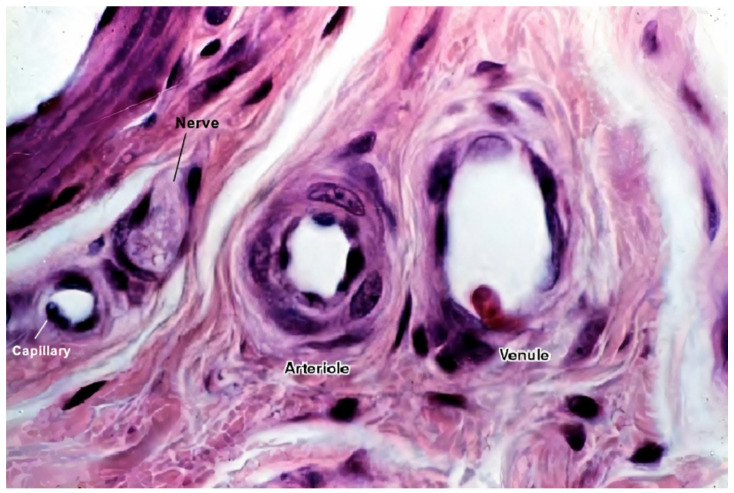
\includegraphics[scale=0.7]{gambar/mikrovaskular.jpg}
	\caption{ Sistem Mikrovaskular \cite{guven_microcirculation_2020}}
	\label{fig:mikrovaskular}
\end{figure}


\noindent Mikrovaskular merupakan cabang terkecil dari pembuluh darah, memainkan peran penting dalam sirkulasi darah dan pertukaran zat di seluruh tubuh \cite{rusanova_role_2022}. Struktur ini, dengan ukuran kurang dari 100 mikrometer, terdiri dari arteriol, kapiler dan venula \cite{mescher_junqueiras_2021,pepe_microvascular_2023}. Arteriol merupakan pembuluh darah berdiameter 10-100 $\mu$m yang bertindak sebagai pengatur tekanan darah. Kapiler merupakan pembuluh darah berdiameter 4-10 $\mu$m yang berfungsi sebagai tempat pertukaran metabolit antara darah dan jaringan \cite{haffner_emerging_2023}. Venula merupakan pembuluh darah berdiameter 10-100 $\mu$m tempat berlanjutnya aliran darah dari kapiler dan membawanya ke vena. Struktur ini juga berperan sebagai tempat keluarnya leukosit (sel darah putih) untuk mengatasi infeksi atau peradangan pada jaringan.


\noindent Studi tentang mikrovaskular sangat penting dalam bidang kesehatan dan patologi. penelitian internasional yang sedang berlangsung \textit{Human Cell Atlas }(HCA) oleh Chan Zuckerberg Initiative, \textit{Human Protein Atlas} (HPA) oleh Knut and Allice Wallenberg Foundation dan \textit{Human BioMolecular Atlas Program} (HuBMAP) oleh National Institutes of Health menggunakan kerangka kerja yang bernama \textit{Vascular Common Coordinate Framework} (VCCF) yang memanfaatkan pembuluh darah sebagai sistem koordinat dalam tubuh manusia untuk memetakan setiap sel di seluruh tubuh manusia \cite{weber_considerations_2020,zhao_attention-based_2023}. penelitian tersebut dilakukan untuk memahami spesialisasi, interaksi dan organisasi spasial setiap sel dalam tubuh manusia.

\noindent Pemanfaatan mikrovaskular sebagai kordinat pada kerangka kerja VCCF tersebut bisa dilakukan karena pembuluh darah  mengikuti setiap jalur unik di setiap organ sehingga bisa mencerminkan sifat biologis khusus setiap jaringan \cite{weber_considerations_2020}. Kerumitan struktur mikrovaskular mencerminkan kompleksitas organ dan jaringan yang dilaluinya, sehingga dapat menyoroti ketergantungan antara mikrovaskular dan sel dalam menjalankan fungsi yang tepat. 



\section{Ginjal dan Mikrovaskular Ginjal}


Ginjal adalah organ vital yang bertanggung jawab untuk menyaring darah, mengatur tekanan darah, dan menjaga keseimbangan elektrolit dalam tubuh manusia \cite{sultan_microvasculature_2023,ito_s-27-1_2023,bagarao_renal_2023}. %+\citeabdulla_biology_2022
Ginjal melakukan hal tersebut melalui proses-proses seperti filtrasi glomelurus, penyerapan tubulus, dan sekresi tubulus, yang pada akhirnya membentuk urin \cite{auctores_publishing_llc_what_2021}. Kemudian, ginjal membantu mengatur volume cairan tubuh, kandungan elekrolit, dan keasaman, serta membuang produk limbah dan racun dalam tubuh. Secara garis besar, ginjal sangat penting untuk menjaga lingkungan internal tubuh, guna menjamin kondisi yang optimal agar berbagai proses tubuh dapat berfungsi dengan baik.
 

\noindent Fungsi-fungsi vital ginjal dilakukan oleh struktur-struktur khusus di dalamnya, terutama pada bagian korteks, medula, dan papila. Masing-masing bagian ini memiliki peran unik dalam proses filtrasi, reabsorpsi dan sekresi yang terjadi di ginjal. korteks merupakan area terluar ginjal yang memiliki sel-sel bulat ginjal yang membungkus glomelurus sebagai alat untuk menyaring darah \cite{gopalan_renal_2022,mescher_junqueiras_2021}. Medula merupakan area dalam dalam ginjal terdiri dari tubulus-tubulus nefron (lengkung Henle dan duktus kolektivus) dan pembuluh struktur kapiler khusus medula bernama vasa recta yang berperan dalam pengatur konsentrasi urin \cite{haug_multi-omic_2022}. Papila merupakan sub bagian dari medula yang merupakan dasar dari piramida ginjal berfungsi sebagai tempat pengumpulan urin sebelum di teruskan ke kaliks minor \cite{sabate_arroyo_relationship_2020}.

\noindent Mikrovaskular ginjal memiliki beberapa komponen unik yang berperan penting dalam proses pembentukan urin dan pengaturan fungsi ginjal, mencakup glomelurus, kapiler peritubular, vasa recta, arteriol aferen dan arteriol eferen \cite{mescher_junqueiras_2021}. Glomelurus merupakan kumpulan kapiler yang terdapat di kapsul Bowman yang berfungsi sebagai alat penyaring darah sehingga air dan limbah bisa melewati dinding kapiler ke dalam kapsul Bowman, sementara sel darah dan protein besar tetap berada di dalam aliran darah \cite{luxen_unique_2023}. kapiler peritubular merupakan kapiler yang mengelilingi tubulus ginjal yang berperan mereabsorsi cairan penting yang tidak tersaring di dalam glomelurus \cite{savedchuk_targeting_2023}. Vasa recta merupakan kapiler yang terletak di medula ginjal, mengelilingi  lengkung henle yang berfungsi menjaga gradien osmotik untuk proses reabsorsi air dari duktus kolektivus \cite{goligorsky_emerging_2022}. Arteriol aferen dan eferen merupakan arteriol  yang berfungsi dalam transportasi darah dari dan ke glomlurus \cite{ergin_kidney_2021}.



\section{Whole Slides Image (WSI)}

\noindent \textit{Whole Slide Image} (WSI) merupakan teknologi dalam pengambilan gambar histologi yang melibatkan pemindaian slide mikroskopik menjadi gambar digital beresolusi tinggi \cite{hanna_whole_2020}. Gambar yang dihasilkan dari pemindaian WSI biasanya berukuran besar (ratusan hingga ribuan megabyte) yang di simpan dalam berbagai format, termasuk \textit{Scope Virtual Slide} (SVS), \textit{MIRAX Slide Image} (MRXS), \textit{NanoZoomer Digital Pathology Image} (NDPI), \textit{Tagged Image File Format} (TIFF), dan \textit{Digital Imaging and Communications in Medicine }(DICOM). Penggunaan WSI dalam pemindaian slide mikroskopik ini dapat meningkatkan reproduksibilitas analisis dan mengurangi kesalahan manusia dalam interpretasi visual \cite{li_hardware-software_2023}. Dalam dunia patologi WSI juga dimanfaatkan untuk berbagai keperluan termasuk: diagnosis primer dimana dalam pembuatan diagnosis tanpa melihat ke dalam slide kaca secara langsung, konsultasi jarak jauh dengan berbagai WSI secara digital dan penelitian yang melibatkan analisis WSI untuk penelitian biomolekular, penemuan obat baru dan pengembangan alat diagnostik.

\begin{figure}[h]
	\centering
	\begin{subfigure}[b]{0.3\textwidth}
		\centering
		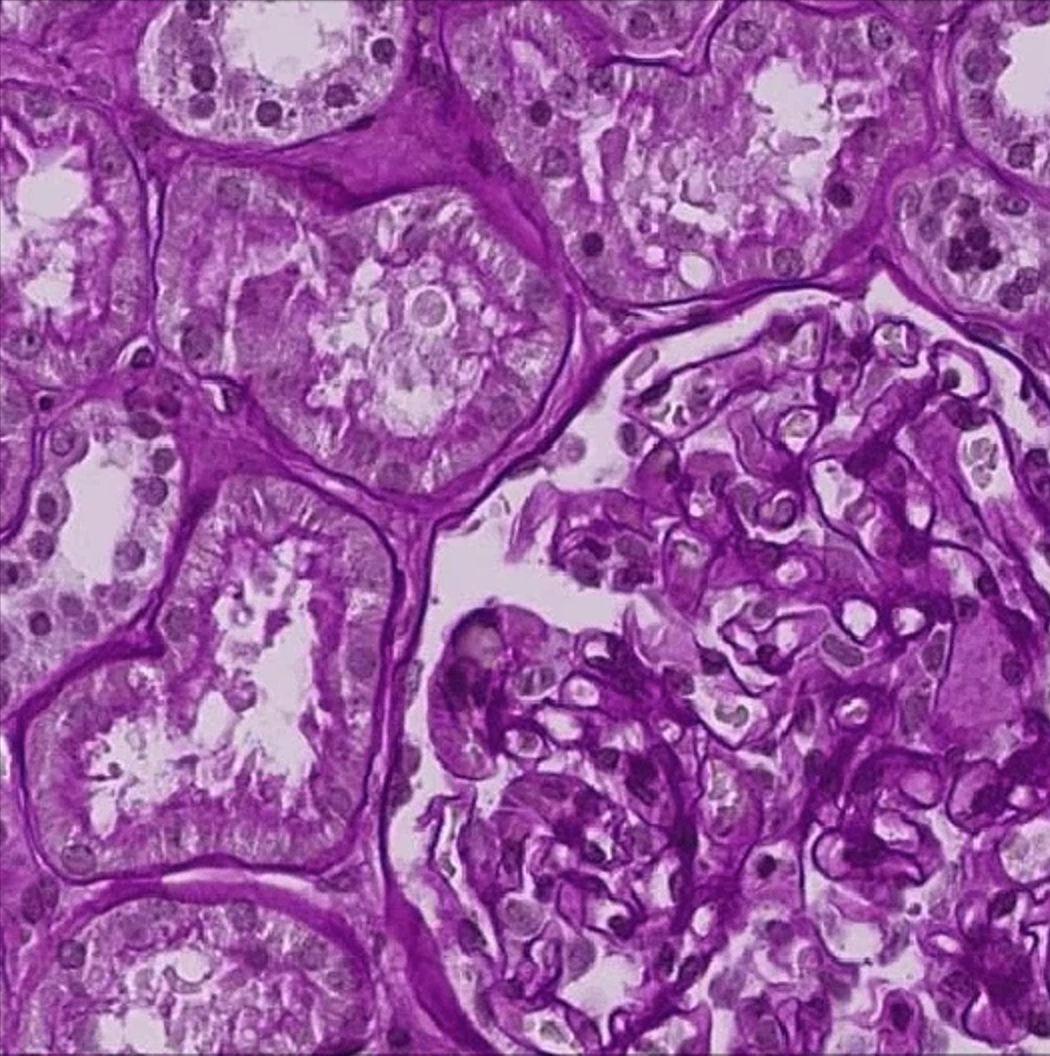
\includegraphics[width=\textwidth]{gambar/korteks.png}
		\caption{Korteks}
		\label{fig:korteks}
	\end{subfigure}
	\hfill
	\begin{subfigure}[b]{0.3\textwidth}
		\centering
		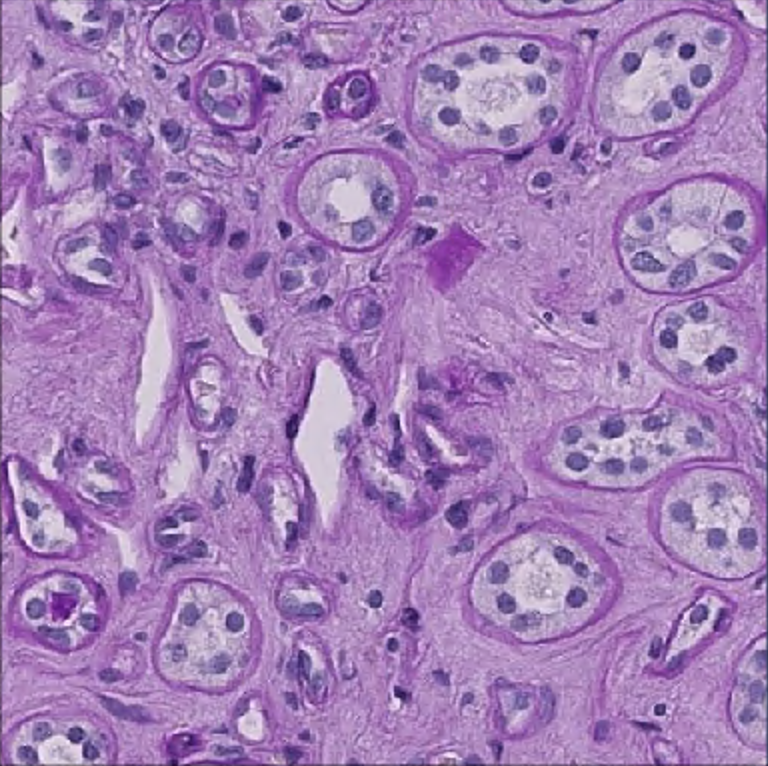
\includegraphics[width=\textwidth]{gambar/medula.png}
		\caption{Medula}
		\label{fig:medula}
	\end{subfigure}
	\hfill
	\begin{subfigure}[b]{0.3\textwidth}
		\centering
		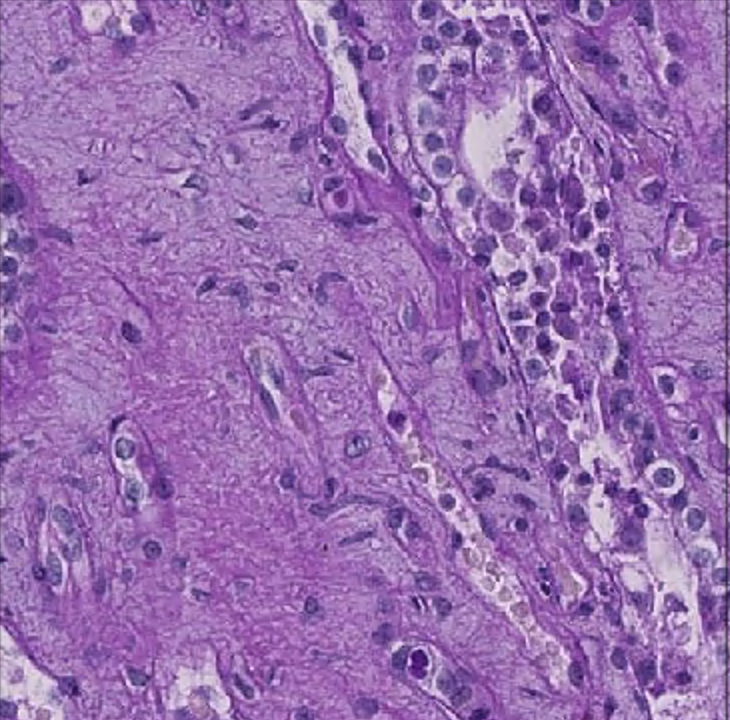
\includegraphics[width=\textwidth]{gambar/papila.png}
		\caption{Papila}
		\label{fig:papila}
	\end{subfigure}
	\caption{Sample WSI pada bagian ginjal \cite{howard_hubmap_2023}}
	\label{fig:ginjal}
\end{figure}

 
\section{Segmentasi Gambar}

\noindent Segementasi gambar merupakan sebuah tugas penting dalam anilisis gambar histologis dan medis. Proses ini akan mempartisi gambar digital menjadi wilayah yang terpisah (tidak tumpang tindih), yang masing-masing wilayah  berhubungan dengan suatu objek atau struktur yang relevan dalam lingkup pengamatan \cite{wu_image_2023}. Dengan kata lain, segmentasi gambar merupakan proses mengelompokkan piksel-piksel dalam gambar berdasarkan karakteristik tertentu. Hasil dari segmentasi gambar adalah sekumpulan segmen yang mewakili objek dari objek yang berbeda dalam gambar. Metode yang di gunakan dalam proses ini sangat bervariasi, dari yang metode sederhana seperti: \textit{treshholding} memisahkan piksel berdasarkan intensitasnya, \textit{region growing} mengelompokkan piksel-piksel berdasarkan kemiripan, \textit{clustering} memisahkan piksel berdasarkan kemiripan dalam fitur multidimensi dan \textit{aktive countour} menggunakan kurva yang dapat berubah untuk mendeteksi objek, hingga metode \textit{deep learning} seperti model FCN yang lebih canggih \cite{huang_fully_2022,wang_comprehensive_2022}.

\noindent Dalam praktiknya segmentasi gambar menggunakan \textit{deep learning} terbagi ke dalam dua jenis: segmentasi semantik dan segmentasi instance. Segmentasi semantik merupakan jenis segmentasi untuk mencari pemahan rinci terhadap berbagai wilayah dalam gambar yang mana pada jenis ini pelabelan setiap piksel dalam gambar didasarkan setiap kelas objek \cite{fan_image_2023}. Di sisi lain, segmentasi instace melabeli piksel objek dalam gambar tidak hanya didasarkan setiap kelas dari objek tetapi, juga membedakan antara instance objek  secara individu walaupun ada dalam kelas yang sama sehingga memungkinkan untuk penggambaran yang tepat dari setiap objek yang ada dalam gambar. Kedua jenis segmentasi ini telah dimanfaatkan dalam berbagai bidang seperti analisis citra lalulintas untuk sistem kemudi otomatis, transfer gaya gambar dalam komputer vision dan analisis struktur mikrovaskular sebagaimana yang akan dilakukan pada penelitian ini \cite{wang_traffic_2023, zhang_image_2023, sultan_microvasculature_2023}


\section{Deep Learning}

\noindent Deep learning merupakan sub bidang dari machine learning yang menggunakan jaringan syaraf tiruan dengan banyak layer untuk mempelajari pola dari suatu data \cite{goodfellow_deep_2016,yang_deep_2023}. Perkembangan deep learning memberikan pengaruh besar pada analisis citra medis \cite{sistaninejhad_review_2023}. Dimana pada tahap awal perkembangan analisa citra medis, fitur-fitur diektraksi secara tradisional menggunakan teknik pemrosesan citra tradisional yang memakan waktu dan butuh validasi ahli \cite{huang_fully_2022}.  Kemudian, dengan munculnya deep leaning terutama \textit{Convolutional Neural Network} (CNN), proses ektraksi fiturpun menjadi otomatis \cite{huang_fully_2022,azad_medical_2022}. 

\begin{figure}[H]
	\centering
	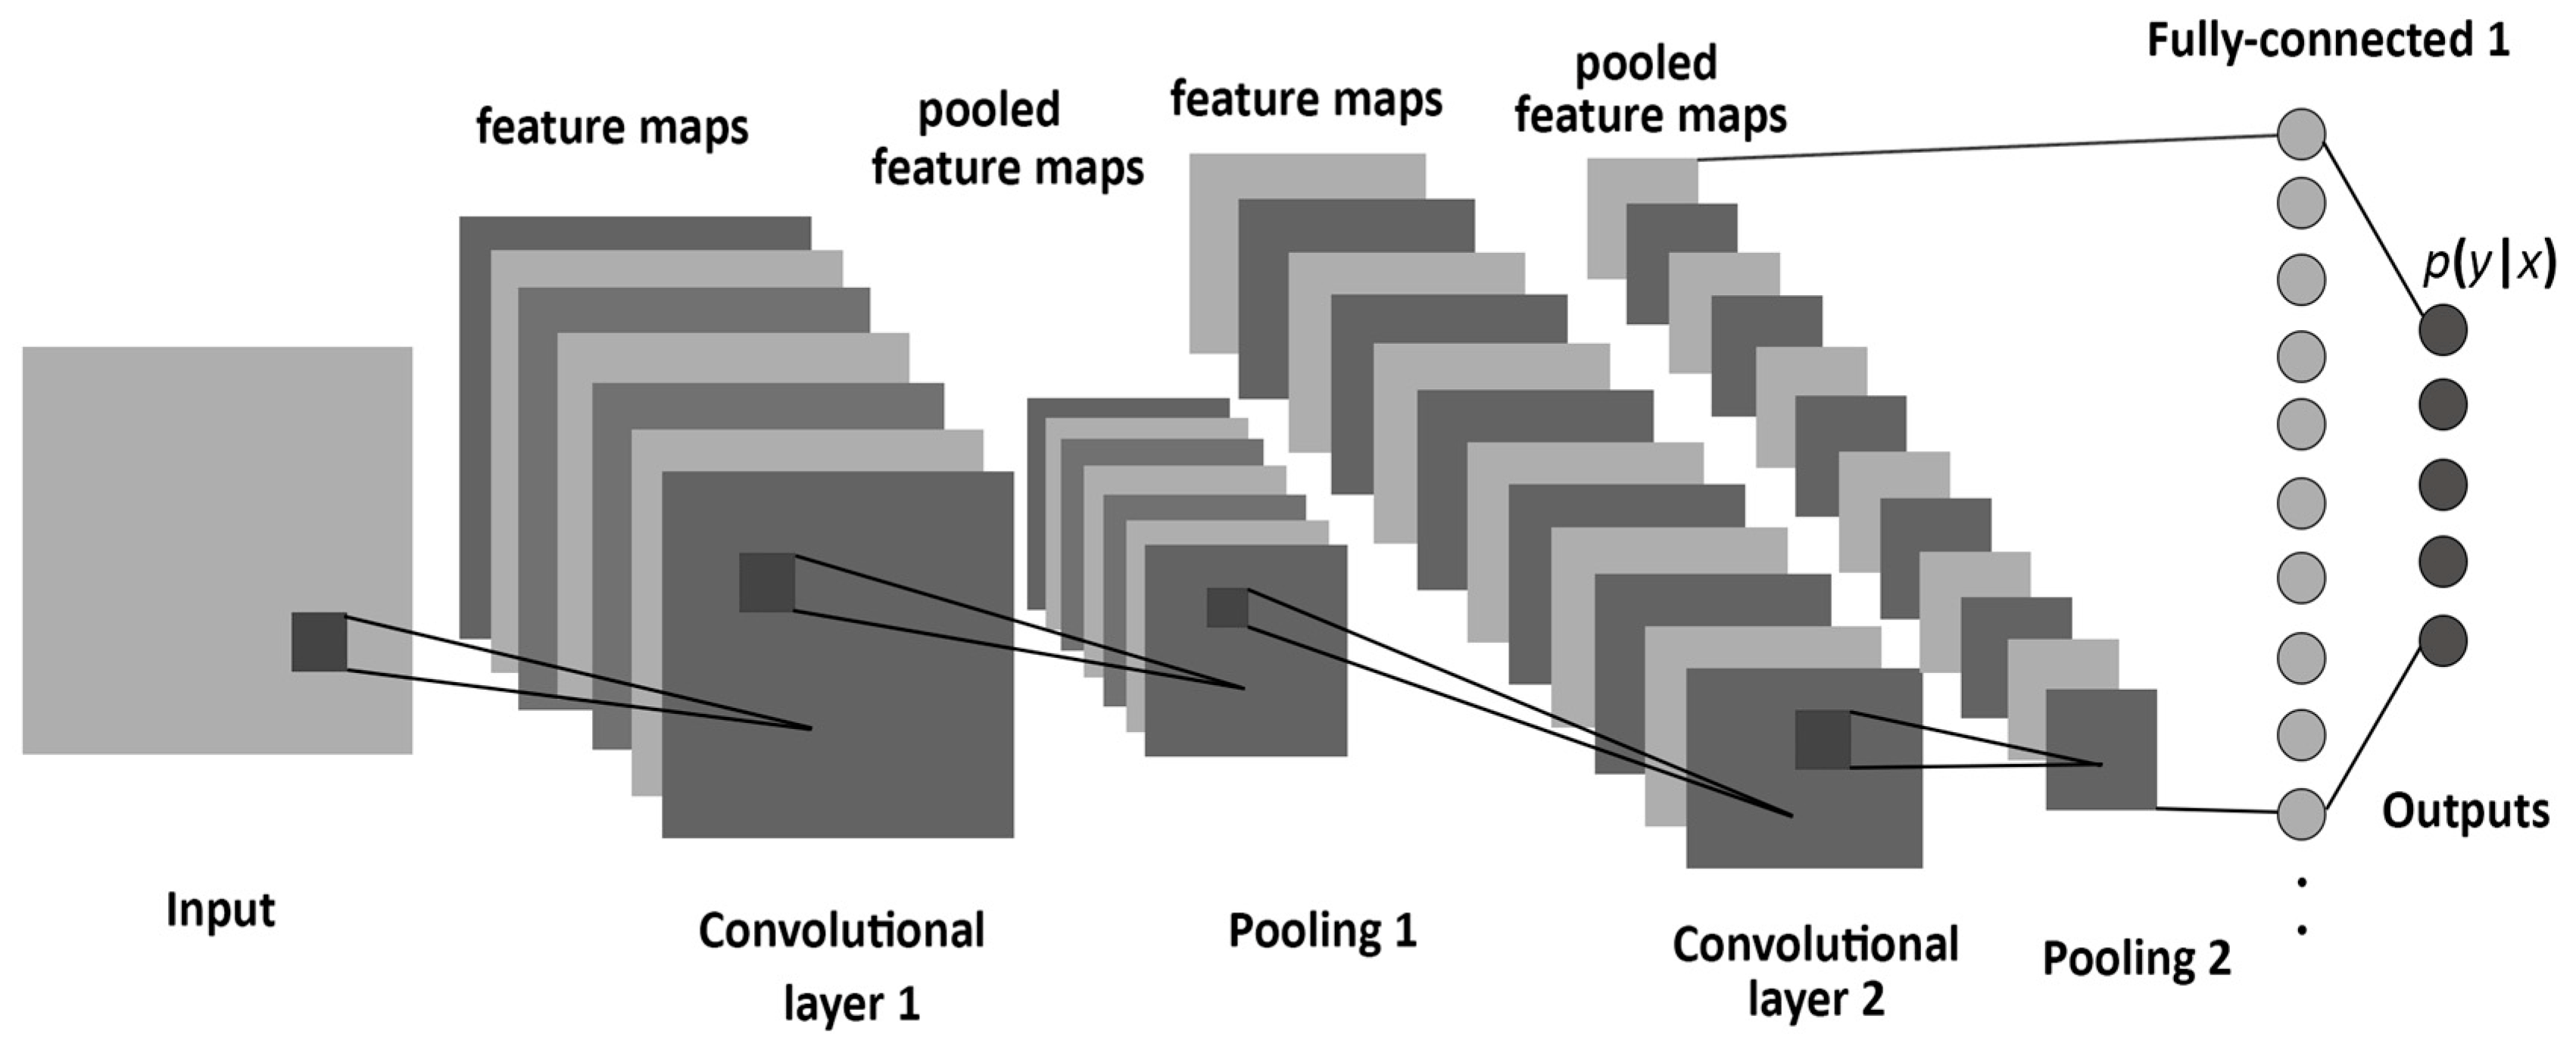
\includegraphics[scale=.08]{gambar/CNN.PNG}
	\caption{Model CNN \cite{albelwi_framework_2017}}
	\label{fig:CNN}
\end{figure}

\noindent CNN merupakan model jaringan saraf tiruan yang sangat efektif untuk tugas-tugas pengolahan citra, seperti klasifikasi gambar dan objek deteksi pada gambar \cite{celeghin_convolutional_2023}. CNN bekerja dengan cara mengekstraksi fitur-fitur penting dari gambar melalui serangkaian lapisan konvolusi, \textit{pooling}, dan fungsi aktivasi, yang memungkinkan model untuk mengenali pola dan struktur dalam data visual. Namun CNN tradisional memiliki keterbatasan untuk tugas segmentasi  gambar \cite{huang_fully_2022, azad_medical_2022, jasim_towards_2023}. Salah satunya berkaitan dengan fitur yang di ekstraksi model tersebut. Ketika menggunakan kernel yang lebih kecil, fitur yang di hasilkan akan lebih lokal terhadap gambar asli, sehingga informasi global seperti lokasi mungkin hilang. Namun, ketika menggunakan kernel yang lebih besar, konteks dari fitur lokal tersebut dapat berkurang. Untuk mengatasi masalah tersebut Long et al. (2014) \cite{long_fully_2014} memperkenalkan model \textit{Fully Convolutional Network} (FCN) yang lebih cocok untuk tugas segmentasi, karena terdiri dari struktur \textit{encoder-decoder} untuk secara bertahap mengurangi resolusi gambar (downsampling) dan kemudian meningkatkannya kembali (upsampling), memungkinkan model untuk menangkap fitur pada berbagai skala dan mempertahankan informasi spasial.


\subsection{Fully Convolutional Network (FCN)}

Salah satu model \textit{deep learning} yang sering digunakan dalam tugas segmentasi merupakan \textit{Fully Convolutional Network }(FCN). Perbedaan utama antara \textit{Convolutional Neural Network} (CNN) tradisional dan FCN terletak pada lapisan terakhir. CNN tradisional menggunakan \textit{fully connected layer} atau jaringan dense untuk mengintegrasikan informasi sebelum menghasilkan output. Sebaliknya, FCN mengganti lapisan terakhir tersebut dengan jaringan konvolusi untuk menghasilkan output channel \cite{shlezinger_model-based_2023,huang_fully_2022}. Salah satu manfaat utama dari pendekatan ini adalah bahwa model tidak akan mendapatkan pembatasan dari \textit{fully connected layer}, sehingga ukuran dari output	 akan lebih fleksibel \cite{iqbal_analyses_2023}.


Struktur FCN seperti pada gambar \ref{fig:fcn} menerapkan beberapa blok konvolusi yang terdiri dari lapisan konvolusi, aktivasi dan \textit{pooling} pada jalur encoder untuk menangkap representasi semantik dari gambar \cite{azad_medical_2022}. Begitu juga, dalam jalur decoding FCN menggunakan lapisan konvolusi bersamaan dengan operasi \textit{upsampling} untuk memberikan prediksi pada tingkat piksel sehingga model bisa melakukan tugas segmentasi \cite{deng_fcn_2023}. \textit{Skip conections} juga digunakan dalam FCN untuk menemukan lokasi dari fitur di keseluruhan citra. 

\begin{figure}[H]
	\centering
	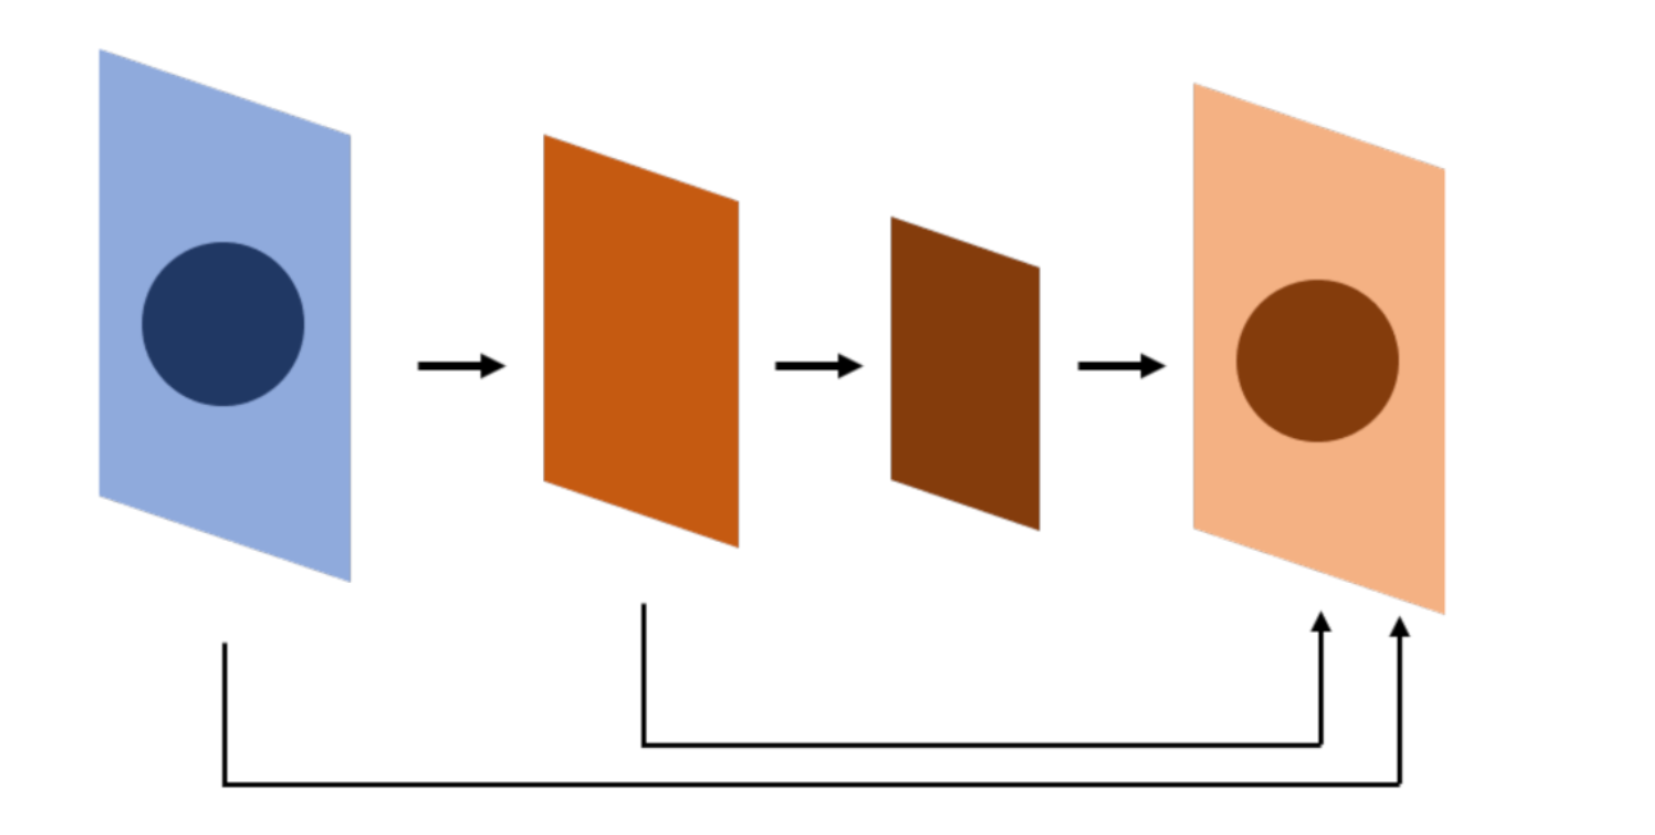
\includegraphics[scale=.2]{gambar/gambar-fcn.png}
	\caption{Model FCN yang bagian terakhirnya di gantikan dengan blok konvolusi \cite{huang_fully_2022}}
	\label{fig:fcn}
\end{figure}


\subsection{U-Net}

\noindent Arstitektur FCN yang terdiri dari bagian \textit{encoder-decoder}, khusus digunakan dalam tugas segmentasi citra biomedis adalah U-Net yang pertama kali dikenalkan oleh Ronneberger et al.(2015) \cite{ronneberger_u-net_2015}. Arsitektur ini menjadi cukup populer di kalangan peneliti, terutama bidang analisis citra biomedis, karena kemampuannya untuk memberikan hasil segmentasi yang akurat dengan jumlah data pelatihan yang relatif kecil \cite{williams_unified_2023}.

\begin{figure}[H]
	\centering
	\includegraphics[scale=.2]{gambar/U-Net.png}
	\caption{Arsitektur dasar U-Net yang digunakan untuk tugas segmentasi citra biomedis \cite{ronneberger_u-net_2015}}
	\label{fig:U-net}
\end{figure}

\noindent U-Net memanfaatkan ekstraksi fitur dari jaringan konvolutional, dimana lapisan \textit{upsampling} dan \textit{skip connection} digunakan untuk membandingkan fitur dari lapisan atas sambil tetap mempertahankan fitur dari lapisan bawah \cite{huang_fully_2022}. Dengan demikian, model mampu mendeteksi fitur-fitur detail dan umum dari objek, sehingga bisa mendeteksi objek secara akurat. U-Net dapat disebut sebagai metode klasifikasi tingkat piksel, dimana segmentasi dilakukan melalui klasifikasi piksel per piksel \cite{siddique_u-net_2020}. Struktur arsitektur dari U-Net akan dijelaskan secara singkat sebagai berikut:

\begin{itemize}
	\item Bagian pertama dari arsitektur U-Net adalah bagian menurun yang dikenal juga sebagai bagian \textit{encoder} yang berfungsi untuk menangkap informasi kontekstual gambar \cite{azad_medical_2022}. Bagian ini terdiri dari unit-unit blok konvolusi, dimana setiap blok berisi dua \textit{convolution layers} 3x3 berurutan dan \textit{pooling layers} yang mirip dengan CNN konvensional, kadang juga menyertakan juga menyertakan \textit{batch normalization layers} \cite{younisse_fine-tuning_2023}. Sebelum memasuki \textit{pooling layers}, fitur akan difilter terlebih dahulu melalui fungsi aktivasi ReLu untuk menentukan apakah fitur yang diekstraksi akan ditransfer ke layer selanjutnya.
	
	\item Bagian kedua adalah bagian mendaki yang dikenal juga sebagai bagian \textit{decoder} yang bertujuan untuk secara bertahap meningkatan pemetaan fitur ke resolusi yang diinginkan\cite{siddique_u-net_2020}. Bagian ini terdiri dari layer \textit{transpose convolution} 2x2 (atau deconvolution) yang berfunsi sebagai \textit{upsampling} untuk mengembalikan dimensi spasial yang hilang selama proses pooling pada bagian encoder. Kemudian, diikuti dua \textit{convolution layers} 3x3 berurutan untuk memperbaiki fitur yang telah di-\textit{upsampling} untuk memastikan detail spasial tetap terjaga dan diperbaiki\cite{purushothaman_image_2022}. Fungsi aktivasi ReLu juga digunakan pada bagian ini setelah setiap operasi konvolusi untuk memperkenalkan non-linieritas yang memungkinkan jaringan untuk mempelajari representasi yang lebih kompleks dan akurat pada resolusi yang lebih tinggi\cite{huang_fully_2022}.
	
	\item Diantara \textit{encoder} dan \textit{decoder} terdapat \textit{bottleneck} yang terdiri dari \textit{convolution layers} 3x3 berurutan dengan fungsi aktivasi ReLu \cite{azad_medical_2022}. Bagian ini berfungsi untuk menangkap fitur pada resolusi terendah dan menghubungkan informasi dari \textit{encoder} dan \textit{deceoder}.
	
	\item \textit{Skip connection} dari \textit{encoder} ke \textit{decoder} digunakan juga pada U-Net untuk meningkatkan kinerja model pada tugas segmentasi gambar \cite{azad_medical_2022}. \textit{Skip connection}  merupakan jalur langsung yang menghubungkan layer pada bagian \textit{encoder} dengan layer pada bagian \textit{decoder} pada tingkat resolusi yang sama. Dengan penggunaan \textit{skip connection} memungkinkan model untuk mempertahankan fitur resolusi tinggi dari gambar input yang mungkin hilang selama proses \textit{downsampling} di \textit{encoder}. Kemudian,\textit{ skip connection} juga mepertahankan informasi lokasi yang membantu dalam rekontruksi fitur yang lebih akurat\cite{siddique_u-net_2020}.
	
	\item \textit{Output layers}  pada arsitektur U-Net ini merupakan sebuah \textit{convolutional layer} 1x1 yang berada di puncak decoder berfungsi untuk menghasilkan prediksi piksel per piksel \cite{huang_fully_2022,azad_medical_2022}. Fungsi aktivasi Softmax sering diterapkan pada layer output untuk menghasilkan distribusi probabilitas setiap kelas pada setiap piksel. Namun, untuk data yang terdiri dari dua kelas lebih umum digunakan fungsi aktivasi sigmoid.
	
	
\end{itemize}



\section{Modul Attention Gate (AG)}

\noindent Penggunaan modul \textit{Attention Gate} (AG) pertamakali digunakan dalam \textit{deep learning} di pemrosesan bahasa alami (natural language proccessing)\cite{azad_medical_2022}. Modul ini mencari korelasi antara query dan key untuk mendapatkan bobot yang sesuai dengan kata kunci. Hasilnya, AG ini dapat menangkap hubungan antara teks dalam suatu wilayah atau paragraf dengan lebih tepat. Konsep serupa juga bisa digunakan dalam \textit{computer vision} \cite{huang_fully_2022}. Menerapkan AG dapat membuat model menggabungkan korelasi fitur-fitur regional, sehingga menghasilkan hasil deteksi tepi objek yang lebih baik untuk meningkatkan kinerja.



\noindent Citra biomedis memiliki variasi tinggi dalam bentuk dan ukuran. Pendekatan umum yang biasanya dilakukan untuk menghadapi masalah ini adalah susunan \textit{cassaded network}, dimana jaringan pertama  mengekstraksi \textit{region of interest} (ROI) termasuk organ yang akan di segmentasi, dan jaringan kedua meprediksi segmentasi organ yang tepat di dalam ROI \cite{oktay_attention_2018}. Namun, pendekatan ini sering mengalami redudansi parameter model dan kebutuhan sumber daya komputasi yang tinggi. Dengan menambahkan AG pada U-Net seperti pada gambar \ref{fig:Attention-U-net}, model dapat secara efektif menekankan fitur-fitur yang relevan tanpa memerlukan jaringan terpisah untuk prediksi ROI, sehingga mengurangi redundansi parameter dan meningkatkan efisiensi komputasi\cite{azad_medical_2022}.

\begin{figure}[H]
	\centering
	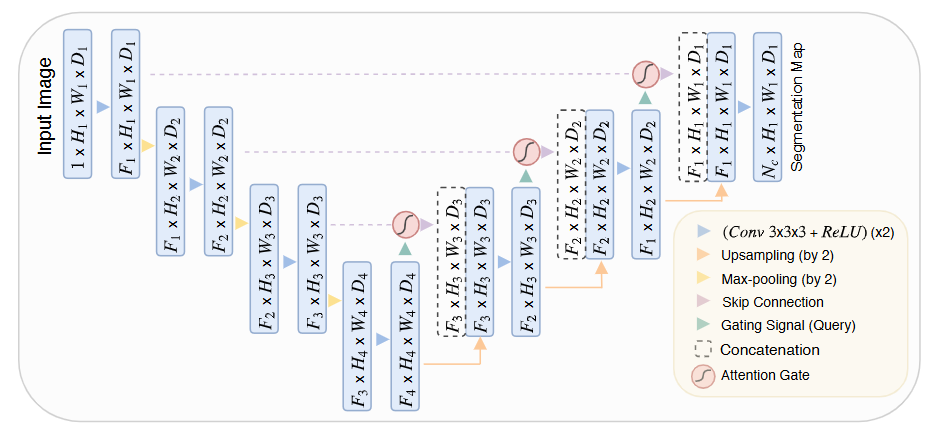
\includegraphics[scale=.5]{gambar/AG-U.png}
	\caption{Diagram Attention U-Net untuk tugas segmentasi \cite{oktay_attention_2018}}
	\label{fig:Attention-U-net}
\end{figure}



Diagram pada gambar \ref{fig:AG} menunjukkan skema kerja AG dalam Attention U-net.AG berfungsi untuk untuk menyoroti fitur-fitur penting yang melewati \textit{skip connections} \cite{siddique_u-net_2020,oktay_attention_2018}. Pertama, fitur input dari layer \(l\) (\(x^l\))  dan sinyal \textit{gating} (\(g\)) yang dikumpulkan dari skala kasar dipetakan ke ruang dimensi yang lebih rendah menggunakan transformasi linier menggunakan konvolusi 1x1x1 secara terpisah. Kemudian, fitur-fitur tersebut ditambahkan dan dilewatkan melalui fungsi aktivasi \textit{Rectified Linear Unit} (ReLU($\sigma1$)) untuk menghasilkan fitur yang lebih terfokus. Setalah itu, hasilnya dilewatkan melalui transformsi linier lain ($\psi$) dengan konvolusi 1x1x1 dan fungsi aktivasi sigmoid ($\sigma1$) untuk mendapatkan koefisien perhatian ($\alpha$). Koefisien perhatian ini kemudian di-resample ke ukuran grid yang sama dengan fitur input asli menggunakan interpolasi bilinier. Fitur input asli \(x^l\) kemudian diskalakan dengan koefisien perhatian yang telah di-resample, menghasilkan output akhir $\hat{x}^l$. Proses ini memastikan bahwa hanya fitur-fitur yang relevan yang diteruskan, sementara yang tidak relevan diabaikan.

\begin{figure}[H]
	\centering
	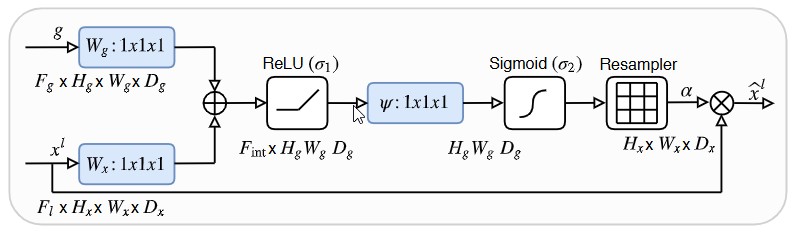
\includegraphics[scale=.5]{gambar/AG.png}
	\caption{Diagram alur kerja Attention Gate \cite{oktay_attention_2018}}
	\label{fig:AG}
\end{figure}

\section{Konvolusi, Pooling dan Transpose Konvolusi}

\noindent Konvolusi, pooling dan transpose konvolusi merupakan lapisan operasi yang digunakan bersama-sama dalam \textit{deep learning}, termasuk U-Net \cite{goodfellow_deep_2016,pajankar_convolutional_2022,bishop_deep_2024}.  Lapisan konvolusi bertindak sebagai pengekstraksi fitur, lapisan pooling berfungsi untuk mengurangi dimensi peta fitur, sedangkan dekonvolusi berfungsi untuk meningkatkan dimensi di bagian \textit{encode}r. 

\subsection{Konvolusi}

\begin{figure}[H]
	\centering
	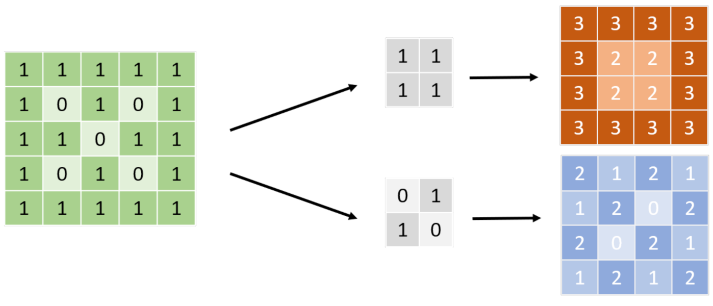
\includegraphics[scale=.3]{gambar/convolusi.png}
	\caption{Penerapan konvolusi terhadap input \cite{huang_fully_2022}}
	\label{fig:convolusi}
\end{figure}

\noindent Konvolusi adalah operasi matematika dimana sebuah kernel (atau filter) digeserkan pada bagian gambar input untuk memproduksi \textit{feature map} (peta fitur) \cite{pajankar_convolutional_2022}.  Pada gambar menunjukkan kernel yang berbeda akan menghasilkan peta fitur yang berbeda juga. Dalam library \textit{deep learning} operasi  konvolusi yang digunakan disebut \textit{cross-corrlelation}\cite{goodfellow_deep_2016}. Dengan formula sebagai berikut:

\begin{equation}
	C(i, j) = (I * K)(i, j) = \sum_{m} \sum_{n} I(i - m, j - n) K(m, n)
\end{equation}


\noindent
keterangan:
\begin{itemize}
	\item $C(i,j)$ : hasil konvolusi pada posisi $(i,j)$
	\item $I(i-m, j-n)$ : nilai piksel citra masukan pada posisi $(i-m, j-n)$
	\item $K(m,n)$ : nilai pada filter di posisi $(m,n)$
\end{itemize}

\subsection{Pooling}

\noindent Fungsi pooling merupakan sebuah fungsi untuk mengubah \textit{output} jaringan di lokasi tertentu menjadi ringkasan statistik dari \textit{output} terdekat\cite{goodfellow_deep_2016,bishop_deep_2024}. Fungsi ini berguna untuk melakukan down-sampling pada peta fitur, yang berarti mengurangi dimensi peta fitur sambil tetap mempertahankan informasi penting. \textit{Down-sampling} ini mengenalkan \textit{invariance} pada jaringan \cite{goodfellow_deep_2016}. Sehingga jaringan bisa melihat fitur mana yang lebih sering muncul, tanpa tergantung pada lokasi aslinya.

\noindent Jenis pooling yang sering digunakan dalam deep learning meliputi \textit{max pooling}, yang mengambil nilai maksimum dari area yang dipilih \cite{bishop_deep_2024}. Kemudian ada \textit{average pooling} yang mengambil rata-rata dari nilai-nilai di area tersebut \cite{bishop_deep_2024}. Dalam arsitektur U-net, \textit{max pooling} digunakan karena efektif dalam mempertahankan fitur-fitur dominan yang penting untuk segmentasi.

\begin{figure}[H]
	\centering
	\includegraphics[scale=0.5]{gambar/figure_8.pdf}
	\caption{Pnerapan pooling terhadap peta fitur \cite{bishop_deep_2024}}
	\label{fig:pooling}
\end{figure}

\subsection{Transpose Konvolusi}


\noindent Transpose konvolusi atau dekonvolusi merupakan fungsi yang digunakan untuk meningkatkan dimensi peta fitur \cite{goodfellow_deep_2016,bishop_deep_2024}. Pada arsitektur U-Net fungsi ini digunakan pada bagian \textit{up-sampling} untuk mengembalikan ukuran peta fitur yang telah melalui bagian \textit{down-sampling} \cite{azad_medical_2022}. Cara kerja operasi ini adalah dengan menerapkan filter yang terhubung dengan satu piksel di tensor input pada patch yang ada di tensor output. Secara matematis proses dekonvolusi dapat dirumuskan sebagai berikut:

\begin{equation}
	I(i,j) = (C * K^T)(i,j) = \sum_{m} \sum_{n} C(m, n) K(i - m, j - n)
\end{equation}

\noindent
keterangan:
\begin{itemize}
	\item $I(i,j)$ : nilai pada posisi $(i,j)$ dari hasil transpose convolution
	\item $C(m,n)$ : nilai pada posisi $(m,n)$ dari input
	\item $K(i-m, j-n)$ : nilai pada posisi $(i-m, j-n)$ dari kernel/filter yang diterapkan terbalik
\end{itemize}


\begin{figure}[H]
	\centering
	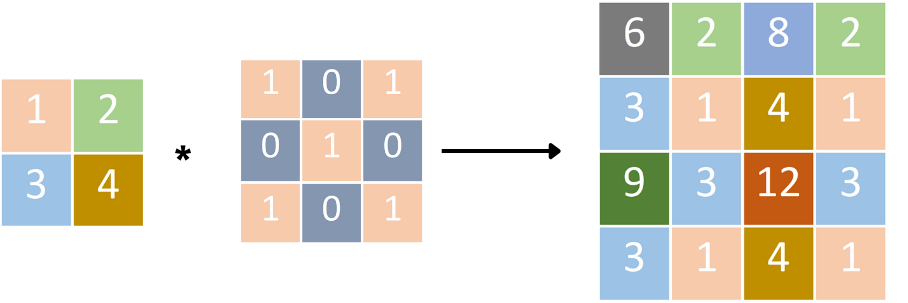
\includegraphics[scale=0.5]{gambar/deconv.png}
	\caption{Transpose konvolusi dari peta fitur \cite{bishop_deep_2024}}
	\label{fig:deconv}
\end{figure}


\section{Augmentasi Data}

\noindent Teknik augmentasi data merupakan salah satu metode yang umum digunakan untuk meningkatkan peforma model deep learning \cite{minaee_image_2020}. Augmentasi data memungkinkan model untuk menghasilkan data baru yang tetap menyerupai data orisinal, tetapi dipandang berbeda oleh model selama pelatihan \cite{huang_fully_2022}. Data augmentasi bisa meningkatkan variasi dari data dan mengurangi gap antara data latih dan uji untuk meningkatkan ketahanan model.

\noindent Dalam pencitraan biomedis augmentasi sering digunakan dalam tugas segmentasi karena ketidakseimbangan antar kelas dalam tugas segmentasi. Oleh karena itu, lebih baik mempertahankan gambar asli fitur untuk konvergensi model. Dalam penerapannya augmentasi biasanya berupa transformasi gemoetris acak (rotation, scaling, shear dan flipping) dan modifikasi intensitas acak (normalization, blurring dan penyesuaian contrast)\cite{minaee_image_2020}.

\section{Oversampling}

\noindent Oversampling merupakan salah satu teknik yang umum dilakukan peneliti dalam menghadapi masalah ketidakseimbangan kelas dalam dataset. Teknik ini bertujuan untuk meningkatkan jumlah sampel dari kelas minoritas dengan mereplikasi sampel-sampel dari kelas tersebut secara acak \cite{bria_addressing_2020}. Dalam konteks segmentasi gambar, oversampling memungkinkan model untuk "melihat" lebih banyak contoh dari objek yang jarang atau kurang terwakili, sehingga model dapat lebih mudah mengenali fitur-fitur dari kelas minoritas. Teknik ini sering dikombinasikan dengan data augmentation yang menambah variasi pada gambar yang dioversample, seperti flipping, rotasi, dan zooming, agar model dapat belajar dengan lebih robust dan menghindari resiko overvitting dari data yang sama.


\section{Fungsi Aktivasi}

\noindent Fungsi aktivasi digunakan dalam \textit{deep learning} untuk memperkenalkan non-linieritas kepada sebuah jaringan, memungkinkan jaringan mengenali kompleksitas dari sebuah data \cite{younisse_fine-tuning_2023,heaton_ian_2018}. Tanpa adanya fungsi aktivasi, jaringan hanya akan menjadi representasi linier dari seluruh data yang dilatih \cite{chiang_activation_2023}. Selain itu, juga akan menyebabkan masalah seperti \textit{vanishing gradient} (gradien yang hilang) atau \textit{exploding gradient} (gradien yang meledak), yang akan menghambat proses pembelajaran jaringan. Salah dua fungsi aktivasi yang sering digunakan dalam arsitektur jaringan U-net adalah \textit{Rectified Linear Unit} (ReLU) dan \textit{sigmoid}. %Penjelasan singkat dari keduanya adalah sebagai berikut ini:

\subsection{ReLU:}
Merupakan singkatan dari \textit{rectified linear unit}. Cara kerja dari fungsi aktivasi ini cukup sederhana, jika input (x) adalah positif maka outputnya adalah nilai itu sendiri \cite{younisse_fine-tuning_2023}. Jika inpuntya negatif atau nol maka outputnya adalah nol. Dengan kata lain, fungsi aktivasi ReLU mengaktifkan neuron dengan input positif dan menonaktifkan selainnya. secara matematis fungsi ReLU adalah sebagai berikut ini: 

\begin{equation}
	\sigma(x) = \max(0, x)
\end{equation}

\noindent
keterangan:
\begin{itemize}
	\item $x$ : nilai piksel setiap \textit{feature map} yang dihasilkan lapisan konvolusi
	\item $\max$ : fungsi yang akan memilih nilai terbesar antara 0 dan nilai $x$
\end{itemize}

\subsection{Sigmoid:}
Merupakan fungsi aktivasi yang memetakan setiap nilai input (x) ke rentang kontitu antara 0 dan 1 untuk melihat ada atau tiadanya sebuah feature \cite{younisse_fine-tuning_2023}. Nilai output akan mendekati 1 untuk input yang sangat besar dan mendekati 0 untuk input yang sangat kecil. Secara matematis fungsi sigmoid dapat didefinisikan sebagai berikut:

\begin{equation}
	\sigma(x) = \frac{1}{1 + e^{-x}}
\end{equation}

\noindent
keterangan:
\begin{itemize}
	\item $x$ : input dari fungsi
	\item $e$ : bilangan \textit{Euler} (bernilai 2.71828)
\end{itemize}


\section{Fungsi Loss}

\noindent Dalam deep learning, pelatihan model merupakan upaya untuk mendekati fungsi sebenarnya dari hubungan kompleks antara input dan output \cite{dawani_hands-mathematics_2020}. Oleh karena itu, fungsi loss diperlukan untuk mengukur seberapa baik kinerja model dalam pelatihan memetakan input ke output yang diinginkan. Pada arsitektur U-Net, loss function yang sering digunakan adalah cross-entropy dan Dice Coefficient \cite{huang_fully_2022}.  

\subsection{Cross-entropy} Fungsi loss ini mengukur perbedaan antara distribusi probabilitas prediksi model dan distribusi probabilitas ground truth \cite{herrera_impact_2022}. Rumusan matematis dari \textit{cross-entropy} adalah sebagai berikut:

\begin{equation} 
	H(p, q) = - \sum_{x} p(x) \log q(x) 
\end{equation} 

\noindent
keterangan:
\begin{itemize}
	\item $p(x)$ : distribusi probabilitas ground truth
	\item $q(x)$ : distribusi probabilitas hasil prediksi oleh model
\end{itemize}

\subsection{Dice coefficient} Fungsi loss ini menghitung area tumpang tindih yang berpasangan antara prediksi segmentasi model dan ground truth, kemudian dibagi dengan piksel yang sama di setiap pasangan \cite{herrera_impact_2022}. Secara matematis dirumuskan sebagai berikut:

\begin{equation}
	s = \frac{2|X \cap Y|}{|X| + |Y|}
\end{equation}
	
\noindent
keterangan:
\begin{itemize}
	\item $X$ : hasil prediksi oleh model
	\item $Y$ : ground truth
\end{itemize}


\section{Optimizer}
\noindent Tahap pelatihan model deep learning merupakan proses mencari set parameter yang paling benar untuk membuat prediksi yang efektif \cite{dawani_hands-mathematics_2020, bishop_deep_2024}. Optimizer pada tahap pelatihan berfungsi untuk mengoptimalkan bobot (weight) dan bias dalam model berdasarkan nilai error yang dihasilkan pada layer output.  Penelitian ini tertarik pada \textit{Stochastic gradient descent} (SGD) dan Adam. Dimana SGD digunakan pada \textit{breaktrough} U-Net oleh Ronnberger et al. (2015) \cite{ronneberger_u-net_2015}. Pada SGD, parameter model diperbarui berdasarkan gradien yang dihitung dari subset data acak dari dataset pelatihan. Adam memberikan hasil pelatihan yang baik pada penelitian tentang \textit{fine-tuning} U-Net oleh Younise et al. (2023) \cite{younisse_fine-tuning_2023}. Adam menggunakan gradien kuadrat untuk menyesuaikan learning rate dan momentum untuk mempercepat konvergensi dengan mengakumulasi gradien sebelumnya.

\section{Hyperparameter}
\noindent Dalam konteks \textit{deep learning}, \textit{hyperparameter} merujuk kepada parameter-parameter yang tidak akan diupdate model selama pelatihan \cite{yu_hyper-parameter_2020}.  Sehingga, parameter-parameter ini harus di tentukan sebelum pelatihan dilakukan. \textit{Hyperparameter} tersebut mongontrol perilaku dari algoritma pelatihan yang memiliki dampak penting terhadap kecepatan dan akurasi pelatihan \cite{goodfellow_deep_2016}.  

\subsection{Learning rate(RL)}
\noindent Learning rate(RL) merupakan seberapa besar perubahan pada parameter model setelah setiap update pada proses pelatihan. LR yang kecil akan memeperlambat pelatihan model sedangkan LR yang besar bisa menyebabkan model terjebak di minimum lokal. Untuk menemukan LR yang optimal merupakan tugas yang sulit dan memerlukan banyak ekperiment sehingga, Wu et all. (2019) \cite{wu_demystifying_2019}, menjelaskan default LR kecil 0.001 merupakan \textit{not bad policy}.

\subsection{Batch size }
\noindent Batch size atau mini batch merujuk kepada banyak sample data yang digunakan dalam setiap iterasi \cite{devarakonda_adabatch_2017}.  Batch size yang besar cenderung menghasilkan estimasi gradien yang lebih stabil tetapi membutuhkan lebih banyak memori, sementara batch size yang lebih kecil membutuhkan lebih sedikit memori namun dapat menghasilkan gradien yang lebih bising \cite{goodfellow_deep_2016}. Untuk efisiensi penggunaan perangkat keras, pemilihan ukuran batch size biasanya menggunakan pangkat 2(contoh: 64, 128, 256, ... )\cite{bishop_deep_2024}.

\subsection{Jumlah epoch}
\noindent Jumlah epoch mengacu pada berapa kali seluruh dataset dilalui selama pelatihan. Terlalu sedikit epoch dapat menyebabkan model underfitting karena tidak cukup belajar dari data, sedangkan terlalu banyak epoch dapat menyebabkan overfitting, di mana model belajar terlalu detail pada data pelatihan dan kehilangan kemampuan untuk menggeneralisasi pada data yang belum pernah dilihat \cite{goodfellow_deep_2016}.

\section{Plateau dalam Pelatihan Deep Learning}

\noindent \textit{Plateau} merupakan keadaan dimana model mengalami stagnasi selama proses pelatihan. Nilai loss (baik training maupun validation loss) tidak menunjukkan perubahan yang signifikan meskipun pelatihan terus berlanjut  dalam beberapa epoch \cite{ainsworth_plateau_2020}.  Keadaan ini dapat disebabkan oleh beberapa faktor, antara lain: 

\begin{itemize}
	\item \textit{Learning  rate} yang terlalu besar atau kecil.
	\item Kompleksitas data yang tinggi, membuat model sulit keluar dari minimum lokal.
	\item Kapasitas model mungkin tidak cukup untuk menangkap pola lebih kompleks dalam data.
\end{itemize}

\noindent Salah satu praktik yang bisa digunakan untuk mengatasi plateau ini adalah penyesuaian learning rate menggunakan \textit{ReduceLROnPlateau callback} dari \textit{library} \textit{Keras} yang akan menyesuaikan laju pembelajaran ketika validation loss berhenti membaik untuk jangka waktu tertentu. Callback ini bertujuan untuk mendorong model keluar dari kondisi stagnasi melalui penyesuaian learning rate.

\section{Metriks Evaluasi}
\noindent Kinerja tugas segmentasi dari jaringan dievaluasi secara kuantitatif menggunakan \textit{intersection over union }(IoU) dan \textit{dice similarity coefficient }(DSC) \cite{jiang_iu-net_2023}. IoU dan DSC digunakan untuk mengevaluasi kemiripan antara hasil segmentasi dan ground truth, dimana semakin mendekati IoU dan DSC dengan 1 maka semakin dekat prediksi dengan ground truth. %Penjelasan dari setiap metriks yang digunakan adalah sebagai berikut ini:

%\subsection{Precission:}
%\noindent Merupakan metriks yang digunakan dalam pengukuran proporsi prediksi yang benar (true positive) dari semua prediksi positif yang dihasilkan model \cite{jiang_iu-net_2023}. Dalam tugas segmentasi, \textit{precision} mengukur seberapa banyak piksel yang diprediksi merupakan bagian dari objek yang benar termasuk kedalam objek tersebut. secara matematis \textit{precision} dapat dirumuskan sebagai berikut:

%\begin{equation}
%	\text{Precision} = \frac{TP}{TP + FP}
%\end{equation}

%\noindent
%keterangan:
%\begin{itemize}
%	\item $TP$ (true positive): jumlah piksel yang benar-benar bagian dari objek dan diprediksi dengan benar sebagai bagian dari objek
%	\item $FP$ (false positive): jumlah piksel yang bukan bagian dari objek namun diprediksi sebagai bagian dari objek
%\end{itemize}

%\subsection{Recall:}
%\noindent Merupakan metriks yang digunakan dalam pengukuran proporsi prediksi benar dari semua prediksi positif yang dihasilkan model \cite{jiang_iu-net_2023}.  Dalam dalam tugas segmentasi, \textit{recall} mengukur seberapa banyak piksel yang prediksi sebagai bagian dari objek benar-benar bagian dari objek tersebut. secara matematis dapat dirumuskan sebagai berikut ini:

%\begin{equation}
%	\text{Recall} = \frac{TP}{TP + FN}
%\end{equation}

%\noindent
%keterangan:
%\begin{itemize}
%	\item $TP$ (true positive): jumlah piksel yang benar-benar bagian dari objek dan diprediksi dengan benar sebagai bagian dari objek
%	\item $FN$ (false negative): jumlah piksel yang merupakan bagian dari objek namun diprediksi sebagai bukan bagian dari objek
%\end{itemize}

\subsection{Intersection over Union (IoU)}
\noindent Merupakan metriks yang digunakan untuk mengukur sejauh mana segmen yang diprediksi oleh model tumpang tindih dengan segmen \textit{ground truth}\cite{jiang_iu-net_2023}. Secara matematis IoU dapat dirumuskan sebagai berikut:

\begin{equation}
	\text{IoU} = \frac{TP}{TP + FP + FN}
\end{equation}

\noindent
keterangan:
\begin{itemize}
	\item $TP$ (true positive): jumlah piksel yang benar-benar bagian dari objek dan diprediksi dengan benar sebagai bagian dari objek
	\item $FP$ (false positive): jumlah piksel yang bukan bagian dari objek namun diprediksi sebagai bagian dari objek
	\item $FN$ (false negative): jumlah piksel yang merupakan bagian dari objek namun diprediksi sebagai bukan bagian dari objek
\end{itemize}

\subsection{Dice Similarity Coefficient (DSC)}

\noindent Merupakan metriks yang digunakan untuk mengukur kesamaan antara segmen yang diprediksi oleh model dan segmen ground truth\cite{jiang_iu-net_2023}. Metrik ini menggunakan faktor dua pada TP sehingga lebih sensitif terhadap kesalah pada area kecil daripada IoU. Secara matematis dapat dirumuskan sebagai berikut:

\begin{equation}
	\text{DSC} =  \frac{2TP}{2TP + FP + FN}
\end{equation}

\noindent
keterangan:
\begin{itemize}
	\item $TP$ (true positive): jumlah piksel yang benar-benar bagian dari objek dan diprediksi dengan benar sebagai bagian dari objek
	\item $FP$ (false positive): jumlah piksel yang bukan bagian dari objek namun diprediksi sebagai bagian dari objek
	\item $FN$ (false negative): jumlah piksel yang merupakan bagian dari objek namun diprediksi sebagai bukan bagian dari objek
\end{itemize}




% Bab 3 metodologi penelitian
\chapter{METODE PENELITIAN}

\noindent Dalam penelitian ini akan dilakukan implementasi model Attention U-net untuk segmentasi mikrovaskular dalam WSI ginjal manusia sehat.  Penggunaan \textit{Aattention Gate} (AG) pada U-net dipilih untuk memusatkan perhatian model pada \textit{feature} yang berpengaruh dari \textit{encoder} ,sehingga bisa meningkatkan peforma model dalam tugas segmentasi mikrovaskular dalam WSI ginjal manusia sehat. Penelitian ini melibatkan beberapa tahapan mulai dari penginputan data sampai ke evaluasi model. Secara mendetail seluruh proses dari penelitian ini bisa dilihat pada flowchart berikut ini:
\begin{figure}[H]
	\centering
	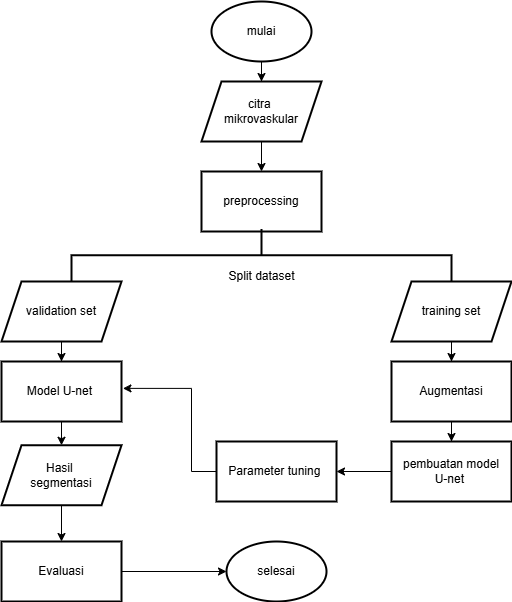
\includegraphics[scale=.6]{gambar/flow-chart.png}
	\caption{Flow chart Penerapan U-net}
	\label{fig:flow-chart}
\end{figure}

\section{Dataset Penelitian}

\noindent Dataset yang digunakan pada penelitian ini adalah data yang telah disediakan \textit{Human BioMolecular Atlas Program }(HuBMAP) di Kaggle: \url{https://www.kaggle.com/competitions/hubmap-organ-segmentation}\cite{howard_hubmap_2023}.  Data ini berisi citra WSL mikrovaskular ginjal manusia yang telah diwarnai menggunakan metode \textit{2D PAS-stained}. \textit{2D PAS-stained} mengacu pada citra dua dimensi yang diwarnai menggunakan pewarnaan Periodic Acid-Schiff (PAS). Data ini terdiri dari 7033 citra yang telah diwarnai dengan format TIFF beresolusi 512x512 dimana 1633 telah dianotasikan ke tiga kelas yakni, \textit{blood vessels}(pembuluh darah), \textit{glomelurus} dan \textit{unsure}(dikeragui).  Anotasi dari data tersebut disimpan dalam file json yang merepresentasikan kordinat mask poligon yang sesuai dengan area setiap kelas pada gambar. Dalam penelitian ini hanya data yang telah dianotasikan saja yang akan digunakan untuk melatih model dengan menggabungkan ketiga kelas anotasi menjadi satu kelas mikrovaskular.

\begin{figure}[H]
	\centering
	\begin{subfigure}[b]{0.3\textwidth}
		\centering
		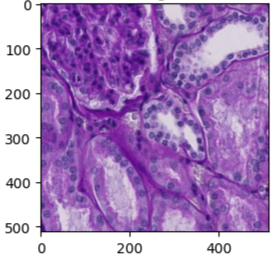
\includegraphics[width=\textwidth]{gambar/image.png}
		\caption{Image}
		\label{fig:image}
	\end{subfigure}
	\hfill
	\begin{subfigure}[b]{0.3\textwidth}
		\centering
		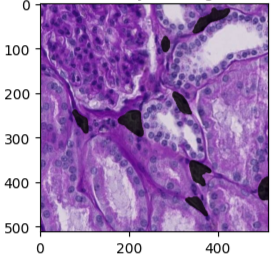
\includegraphics[width=\textwidth]{gambar/overlayed_image.png}
		\caption{Ovelayed image}
		\label{fig:overlayed-image}
	\end{subfigure}
	\hfill
	\begin{subfigure}[b]{0.3\textwidth}
		\centering
		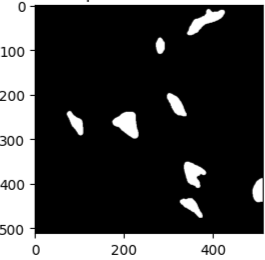
\includegraphics[width=\textwidth]{gambar/pixelwise_label.png}
		\caption{Pixel wise label}
		\label{fig:Pixel wise label}
	\end{subfigure}
	\caption{Sample WSI yang telah dianotasikan}
	\label{fig:sample_data}
\end{figure}

\section{Spesifikasi Perangkat}

\noindent Penelitian ini akan dilakukan di lingkungan komputasi remote menggunakan \textit{Kaggle Notebooks}. Kaggle menyediakan perangkat keras yang diperlukan dalam penelitian, sehingga peneliti bisa fokus pada eksekusi teori ke dalam kode python tanpa perlu konfigurasi perangkat terlebih dahulu. Spesifikasi sumber daya komputasi yang disediakan Kaggle bisa dilihat pada tabel \ref{tab:cpu_specs}.
\begin{table}[h]
	\centering
	\caption{Spesifikasi CPU pada Lingkungan Komputasi Remote Kaggle Notebook.} % caption pakai titik?
	\label{tab:cpu_specs}
	\begin{tabular}{lllll}
		\hline
		\textbf{Jenis} & \textbf{CPU}                             & \textbf{Core CPU} & \textbf{RAM} & \textbf{GPU}        \\ \hline
		CPU            & Default & 4                 & 30 GB        & -                   \\ \hline
		GPU P100       & Intel Skylake                            & 4                 & 29 GB        & 1 Nvidia Tesla P100 \\ \hline
		GPU T4 x2      & Intel Skylake                            & 4                 & 29 GB        & 2 Nvidia Tesla T4   \\ \hline
		TPU 1VM        & -                                        & 96                & 330 GB       & -                   \\ \hline
	\end{tabular}
\end{table}

\noindent \textit{Notebook} yang menggunakan \textit{Central Processing Unit }(CPU) dan \textit{Graphics Processing Unit} (GPU) memiliki waktu eksekusi selama 12 jam, sedangkan notebook yang menggunakan \textit{Tensor Processing Unit} (TPU) memiliki waktu eksekusi selama 9 jam. Tersedia 20 \textit{Gigabytes} ruang penyimpanan otomatis direktori '/kaggle/working' dan ruang penyimpanan \textit{scratchpad} tambahan yang tidak akan disimpan diluar sesi saat ini.


\section{Preproccessing}

\noindent \textit{Preproccessing} merupakan langkah penting dalam mempersiapkan dataset agar bisa gunakan dalam pelatihan dan evaluasi model. Langkah-langkah yang biasanya dilakukan dalam \textit{preproccessing} citra biomedis untuk tugas segmentasi adalah: normalisasi, augmentasi, dan pembagian dataset menjadi data latih dan validasi.

\subsection{Normalisasi}

\noindent Dalam tahap ini, intensitas piksel dari gambar yang biasanya dalam rentang 0 hingga 225 akan di ubah menjadi rentang lebih kecil seperti 0 dan 1. Proses ini bisa mempercepat proses konvergensi model dan meningkatkan akurasi model. Berikut adalah formula untuk normalisasi intensitas piksel dalam gambar:

\begin{equation}
	x' = \frac{x - \min}{\max - \min}
\end{equation}

\noindent
keterangan:
\begin{itemize}
	\item $x$ : nilai piksel asli
	\item $\min$ : nilai minimum dari piksel
	\item $\max$ : nilai maksimum dari piksel
\end{itemize}


\subsection{Pembagian dataset}

\noindent Dalam pengembangan model deep learning pembagian dataset merupakan sebuah langkah yang penting. Dalam langkah ini dataset akan dibagi menjadi set latih dan set uji. Perlakuan ini akan meningkatkan keakuratan evaluasi pada model dengan memastikan model tidak hanya diuji pada data yang telah dilihat selama pelatihan. Rasio pembagian yang digunakan dalam penelitian ini adalah \(80:20\), dimana 80\% data digunakan sebagai set latih dan 20\% data digunakan sebagai set uji. Pembagian ini akan mengambil data secara acak dari seluruh data yang telah dianotasikan saja. 

\subsection{Augmentasi}

\noindent Proses ini merupakan teknik untuk megenerasi  data yang mirip dengan data original namun berbeda pada pandangan model. Pada penelitian ini akan dilakukan augmentasi berupa transformasi geometri secara acak seperti: rotation (rotasi), scaling(skala), shear(geser) dan flipping(membalikkan).

\section{Pelatihan}
Dalam tahap pelatihan citra input dan anotasinya akan digunakan untuk melatih model dengan menuggunakan optimizer Adam dan \textit{Stocastic gradient descent} secara terpisah untuk melihat optimizer mana yang paling cocok dengan model. Kemudian fungsi loss \textit{cross entropy} dan \textit{Dice coefficient loss} akan digunakan secara bersamaan untuk mengatasi masalah ketidakseimbangan kelas dalam pelatihan.


\section{Eksperimen dan evaluasi}

\noindent Dalam tahapan ini akan dilakukan serangkaian eksperimen untuk menjawab pertanyaan permasalahan yang telah dirumuskan. Eksperimen ini dirancang untuk mengevaluasi kinerja model Attention U-net yang diimplementasikan untuk segmentasi mikrovaskular dalam citra WSI ginjal manusia sehat. Berikut adalah berberapa eksperiment yang akan dilakukan dalam penelitian ini:

\begin{itemize}
	\item Model dasar U-net:
	\noindent Eksperimen pertama yang dilakuakan adalah pengimplementasikan model dasar U-net. Model dasar ini juga akan digunakan sebagai titik acuan perbandingan dan evaluasi selanjutnya.
	
	\item Model dasar U-net dengan Augmentasi data:
	\noindent Ekperimen ini akan menambahkan teknik augmentasi data pada model dasar U-net  untuk melihat pengaruh penambahan variasi data peforma model.

	\item Model U-net dengan penerapan Attention Gate:
	\noindent Pada ekperimen ini, attention gate akan ditambahkan ke model U-net untuk menguji pengaruh AG pada peforma model.
	
	\item Model Attention U-net dengan Augmentasi data:
	\noindent Ekperimen ini menggabungkan model Attention U-net dengan teknik augmentasi data untuk mengoptimalkan hasil segmentasi dari Attention U-net.
	
	\item Model dasar FCN:
	\noindent Sebagai tambahan, model dasar FCN juga akan di implementasikan untuk membandingkan peforma segmentasi FCN dengan U-net.
\end{itemize}




% Baris ini digunakan untuk membantu dalam melakukan sitasi
% Karena diapit dengan comment, maka baris ini akan diabaikan
% oleh compiler LaTeX.
\begin{comment}
\bibliography{daftar-pustaka}
\end{comment}


% Bab 4 hasil dan pembahasan
\chapter{HASIL DAN PEMBAHASAN}

\section{Hasil Exploratory Data Analysis}
\label{sec:hasil-eda}

\noindent Tahap Exploratory Data Analysis (EDA) dilakukan untuk memahami karakteristik dataset citra jaringan ginjal secara mendalam. Tujuan utama EDA adalah untuk mengidentifikasi distribusi kelas, mengidentifikasi ketidakseimbangan kelas, dan menemukan pola-pola yang mungkin mempengaruhi kinerja model. Informasi yang diperoleh dari EDA akan digunakan menentukan teknik preprocessing yang tepat pada data sehingga model yang dilatih dapat memberikan hasil yang optimal.

\subsection{Distribusi Citra dalam Dataset}
\noindent Terdapat 1633 citra jaringan ginjal manusia yang telah dilabeli dalam penelitian ini. Citra-citra tersebut terbagi menjadi dua dataset utama. Dataset pertama terdiri dari 2 sumber Whole Slide Imaging (WSI) yang berbeda, sedangkan dataset kedua berasal dari 4 sumber WSI yang berbeda. Diagram di bawah menunjukkan distribusi jumlah citra pada setiap dataset dan kombinasi dataset-sumber WSI.

\begin{figure}[H]
	\centering
	\begin{subfigure}[b]{0.4\textwidth}
		\centering
		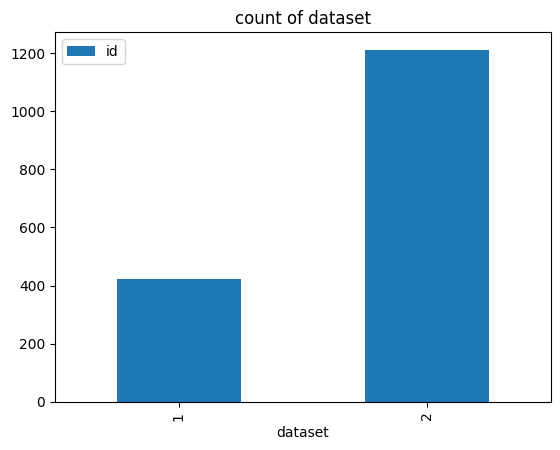
\includegraphics[width=\textwidth]{gambar/bab4/dataset.png}
		\caption{Sebaran citra dalam dataset}
		\label{fig:d_dataset}
	\end{subfigure}
	\hspace{0.05\textwidth}
	\begin{subfigure}[b]{0.4\textwidth}
		\centering
		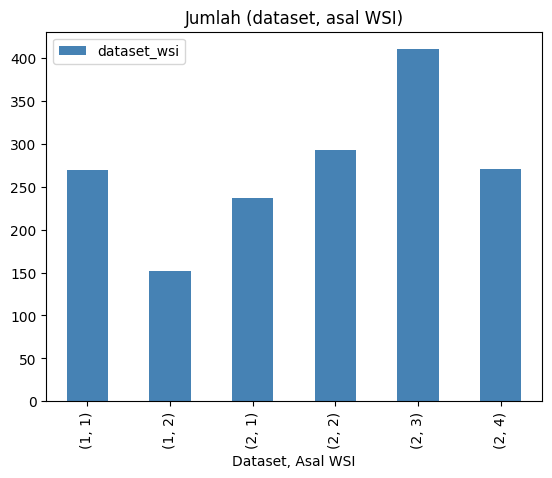
\includegraphics[width=\textwidth]{gambar/bab4/dataset_wsi.png}
		\caption{Sebaran citra dalam sumber WSI}
		\label{fig:d_WSI}
	\end{subfigure}	
	\caption{Sebaran citra pada tiap dataset dan sumber WSI}
	\label{fig:diagram_sebaran}
\end{figure}

\noindent Seperti yang terlihat pada Gambar \ref{fig:d_dataset}, dataset pertama memiliki jumlah citra yang lebih banyak dibandingkan dataset kedua. Sebaran citra pada masing-masing sumber WSI dalam kedua dataset cukup merata setelah ditampilkan berdasarkan asal sumbernya. Selanjutnya, observasi dilakukan untuk menganalisis karakteristik pembuluh darah dari masing-masing sumber WSI pada dataset 1 dan dataset 2 yang bisa dilihat pada lampiran.


\noindent Hasil observasi menunjukkan adanya perbedaan karakteristik pembuluh darah pada dataset 1 yang berasal dari source 1 dan source 2. Pembuluh darah pada source 1 cenderung berjumlah sedikit namun memiliki ukuran yang besar, sedangkan pada source 2, pembuluh darah lebih banyak tetapi berukuran kecil. Sebaliknya, pada dataset 2 yang berasal dari source 1 hingga source 4, tidak ditemukan karakteristik tertentu yang konsisten, karena setiap sampel menunjukkan variasi pembuluh darah yang sangat beragam.

\subsection{Ekplorasi Ukuran Piksel dan Kuantitas Pembuluh Darah}

\noindent Selanjutnya, distribusi ukuran rata-rata (\textit{mean size}) piksel pembuluh darah (dalam ribuan piksel) dan jumlah pembuluh darah (\textit{n$\_$bloodVessel}) untuk setiap sumber dataset dapat dilihat pada Gambar  Scatter plot ini menunjukkan pola distribusi yang berbeda di antara sumber-sumber dataset.

\begin{figure}[H]
	\centering
	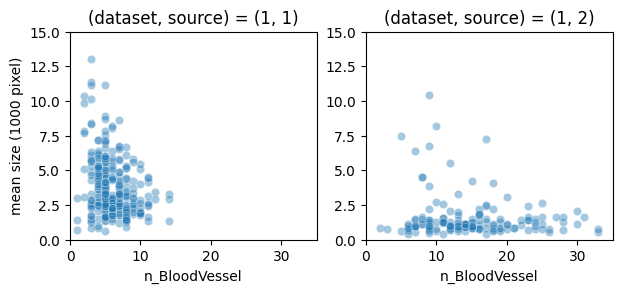
\includegraphics[width=\textwidth]{gambar/bab4/sct_1.png}
	\caption{Sebaran ukuran dan kuantitas pembuluh darah dataset 1}
	\label{fig:sct_1}
\end{figure}

\noindent Pada sumber 1 dan 2, terlihat bahwa jumlah pembuluh darah umumnya berkisar antara 0 hingga 30, dengan ukuran rata-rata piksel pembuluh darah yang cenderung kecil (<5 ribu piksel). Pada sumber 1 terlihat bahwa jumlah pembuluh darah lebih sedikit namun rata-rata piksel pembuluh darah lebih bersar dari sumber 2.

\begin{figure}[h]
	\centering
	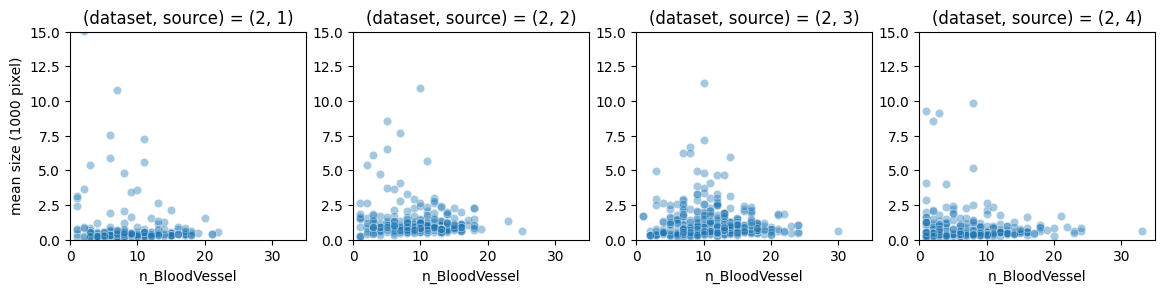
\includegraphics[width=\textwidth]{gambar/bab4/sct_2.png}
	\caption{Sebaran ukuran dan kuantitas pembuluh darah dataset 2}
	\label{fig:sct_2}
\end{figure}

\noindent Distribusi pada dataset 2 lebih beragam dibandingkan dataset 1. Ukuran rata-rata pembuluh darah pada sumber 1 hingga 4 umumnya lebih kecil daripada dataset 1, dengan sebagian besar pembuluh darah berukuran kurang dari 5 ribu piksel.


\subsection{Distribusi label pada dataset}
\noindent Berdasarkan analisis terhadap keseluruhan label dalam dataset, hanya sekitar 5$\%$ label yang merepresentasikan object (pembuluh darah), sedangkan sisanya merupakan latar belakang. Distribusi rata-rata rasio label positif (pembuluh darah) terhadap total label untuk setiap sumber (source WSI) dirangkum pada Tabel berikut:


\begin{table}[H]
	\centering
	\caption{Distribusi rata-rata rasio label positif pada setiap source WSI.}
	\label{tab:distribusi_label}
	\begin{tabular}{cll}
		\hline
		\multicolumn{1}{l}{Dataset} & Source WSI & Positive Ratio \\ \hline
		\multirow{2}{*}{1}          & 1          & 0.083776      \\
		& 2          & 0.084165       \\ \hline
		\multirow{4}{*}{2}          & 1          & 0.024374       \\
		& 2          & 0.048241       \\
		& 3          & 0.047921       \\
		& 4          & 0.023660       \\ \hline
	\end{tabular}
\end{table}

\noindent Dari tabel \ref{tab:distribusi_label} terlihat bahwa distribusi rasio label positif bervariasi antara dataset dan sumber WSI. Dataset 1 memiliki rasio rata-rata label positif yang lebih tinggi (sekitar 8$\%$) dibandingkan dengan dataset 2, di mana rata-rata rasio label positif berkisar antara 2$\%$ hingga 5$\%$. Hal ini menunjukkan adanya ketidakseimbangan kelas yang signifikan dalam dataset, dengan mayoritas piksel pada citra merupakan latar belakang.


\section{Hasil Pelatihan dan Evaluasi}
\noindent Setelah memahami karakteristik dataset melalui Ekplolatory Data Analisys (EDA), model dilatih menggunakan konfigurasi praprosessing dan hyperparameter yang telah ditentukan di Bab \ref{sec:metode-penelitian} Metode Penelitian. Bagian ini akan menyajikan hasil training dan evaluasi model Attention U-Net serta pembandingnya, U-Net, untuk tugas segmentasi mikrovaskular ginjal. Pada tabel \ref{tab:training-results} disajikan seluruh metrik hasil pelatihan.

\begin{landscape}
\begin{table}[]
	\caption{Hasil pelatihan model Attention U-Net dan U-Net dengan berbagai konfigurasi hyperparameter}
	\label{tab:training-results}
	\begin{tabular}{@{}llllllllllll@{}}
		\toprule
		Model &
		Optimizer &
		Batch Size &
		Oversample &
		DSC &
		IoU &
		Recall &
		Precision &
		Train Loss &
		Val Loss &
		Learning Rate &
		Epotch \\ \midrule
		\multirow{10}{*}{Attention U-net} &
		\multirow{5}{*}{SGD} &
		4 &
		Tidak &
		0.362 &
		0.239 &
		0.335 &
		0.488 &
		0.803 &
		0.817 &
		4.0e-5 &
		33 \\
		&  & 8  & Tidak & 0.265          & 0.168          & 0.264          & 0.429          & 0.983 & 1.002  & 2.0e-4 & 49 \\
		&  & 16 & Tidak & 0.181          & 0.113          & 0.152          & 0.445          & 1.027 & 1.055  & 2.0e-4 & 49 \\ \cmidrule(l){3-12} 
		&  & 4  & Ya    & 0.506          & 0.363          & 0.461          & 0.641          & 0.626 & 0.611  & 8.0e-6 & 29 \\
		&  & 8  & Ya    & 0.478          & 0.337          & 0.442          & 0.590          & 0.659 & 0.6441 & 3.2e-7 & 42 \\ \cmidrule(l){2-12} 
		&
		\multirow{5}{*}{Adam} &
		4 &
		Tidak &
		\textbf{0.56} &
		\textbf{0.413} &
		\textbf{0.527} &
		\textbf{0.675} &
		0.53 &
		0.554 &
		1.6e-6 &
		27 \\
		&  & 8  & Tidak & 0.546          & 0.34           & 0.509          & 0.656          & 0.555 & 0.569  & 1.6e-6 & 37 \\
		&  & 16 & Tidak & 0.556          & 0.409          & 0.534          & 0.642          & 0.541 & 0.553  & 8.0e-6 & 29 \\ \cmidrule(l){3-12} 
		&  & 4  & Ya    & \textbf{0.624} & \textbf{0.481} & \textbf{0.595} & \textbf{0.714} & 0.404 & 0.443  & 8.0e-6 & 24 \\
		&  & 8  & Ya    & 0.617          & 0.473          & 0.597          & 0.692          & 0.412 & 0.455  & 8.0e-6 & 25 \\ \midrule
		\multirow{10}{*}{U-net} &
		\multirow{5}{*}{SGD} &
		4 &
		Tidak &
		0.521 &
		0.375 &
		0.48 &
		0.644 &
		0.592 &
		0.601 &
		7.9e-5 &
		25 \\
		&  & 8  & Tidak & 0.396          & 0.268          & 0.346          & 0.572          & 0.764 & 0.767  & 2.0e-4 & 49 \\
		&  & 16 & Tidak & 0.425          & 0.29           & 0.386          & 0.564          & 0.713 & 0.724  & 1.2e-7 & 39 \\ \cmidrule(l){3-12} 
		&  & 4  & Ya    & 0.521          & 0.376          & 0.492          & 0.625          & 0.602 & 0.59   & 1.6e-6 & 38 \\
		&  & 8  & Ya    & 0.510          & 0.367          & 0.475          & 0.620          & 0.598 & 0.605  & 8.0e-6 & 40 \\ \cmidrule(l){2-12} 
		&
		\multirow{5}{*}{Adam} &
		4 &
		Tidak &
		\textbf{0.545} &
		\textbf{0.398} &
		\textbf{0.51} &
		\textbf{0.66} &
		0.557 &
		0.57 &
		1.6e-6 &
		28 \\
		&  & 8  & Tidak & 0.54           & 0.396          & 0.503          & 0.655          & 0.549 & 0.567  & 8.0e-6 & 21 \\
		&  & 16 & Tidak & 0.544          & 0.397          & 0.516          & 0.651          & 0.534 & 0.572  & 1.6e-6 & 36 \\ \cmidrule(l){3-12} 
		&  & 4  & Ya    & \textbf{0.616} & \textbf{0.472} & \textbf{0.59}  & \textbf{0.700} & 0.424 & 0.451  & 3.2e-7 & 29 \\
		&  & 8  & Ya    & 0.612          & 0.467          & 0.593          & 0.687          & 0.432 & 0.456  & 1.6e-6 & 24 \\ \bottomrule
	\end{tabular}
\end{table}
\end{landscape}

\subsection{Hasil Pelatihan Tanpa Oversampling}

\noindent Subbab ini membahas konfigurasi terbaik yang diperoleh pada model Attention U-Net tanpa penggunaan teknik oversampling. Konfigurasi terbaik dipilih berdasarkan nilai train loss dan validation loss terendah, serta pola penurunan loss yang stabil selama pelatihan.

\noindent Berdasarkan hasil eksperimen, konfigurasi terbaik diperoleh dengan optimizer Adam dan batch size 4. Konfigurasi ini menghasilkan train loss sebesar 0.530 dan validation loss sebesar 0.554. Hal ini menunjukkan bahwa konfigurasi ini lebih stabil dibandingkan konfigurasi lain, sebagaimana ditunjukkan pada Gambar \ref{fig:loss_attention_terbaik}.

\begin{figure}[H]
	\centering
	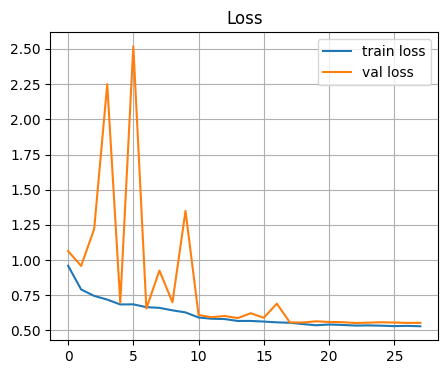
\includegraphics[scale=.8]{gambar/bab4/loss_adam_attention_u-net_4.png}
	\caption{Penurunan training loss dan validation loss pada konfigurasi Attention U-Net terbaik (optimizer Adam, batch size 4).}
	\label{fig:loss_attention_terbaik}
\end{figure}

\noindent Gambar \ref{fig:loss_attention_terbaik} menunjukkan bahwa training loss mengalami penurunan konsisten hingga mencapai konvergensi pada epoch ke-27, dengan learning rate sebesar 1.6e-6. Pola serupa juga terlihat pada validation loss, meskipun terdapat sedikit fluktuasi di epoch awal. Tidak ditemukan indikasi overfitting, karena selisih antara training loss dan validation loss tetap kecil. Penggunaan early stopping membantu menghentikan pelatihan sebelum overfitting terjadi, sehingga validasi tetap konsisten.

\noindent Sebagai perbandingan, konfigurasi dengan optimizer SGD dan batch size 4 menghasilkan train loss sebesar 0.803 dan validation loss sebesar 0.817. Nilai ini lebih tinggi dibandingkan konfigurasi terbaik, menunjukkan bahwa optimizer Adam mampu memberikan stabilitas yang lebih baik dibandingkan SGD. Stabilitas ini didukung oleh kemampuan Adam dalam mengatur gradien selama proses pelatihan.


\subsection{Evaluasi Kinerja Model dalam Segementasi}

\noindent Subbab ini mengevaluasi kinerja model Attention U-Net dan U-Net berdasarkan metrik utama, yaitu Dice Similarity Coefficient (DSC), Intersection over Union (IoU), precision, dan recall. Evaluasi dilakukan untuk berbagai konfigurasi, termasuk variasi batch size dan optimizer, dengan tujuan mengidentifikasi konfigurasi terbaik untuk setiap arsitektur. Tabel \ref{tab:training-results} menyajikan hasil lengkap dari semua eksperimen, di mana performa terbaik ditandai dengan cetak tebal untuk memudahkan interpretasi.

\noindent Berdasarkan hasil pada Tabel \ref{tab:training-results}, model Attention U-Net secara konsisten menunjukkan performa yang lebih baik dibandingkan U-Net pada semua metrik utama. Konfigurasi terbaik untuk Attention U-Net menggunakan optimizer Adam dan batch size 4 menghasilkan DSC sebesar 0.560 dan IoU sebesar 0.413. Sebagai perbandingan, konfigurasi terbaik untuk U-Net (optimizer Adam, batch size 4) hanya mencapai DSC sebesar 0.545 dan IoU sebesar 0.398. Perbedaan ini mengindikasikan bahwa penambahan mekanisme attention gate pada U-Net berkontribusi signifikan dalam meningkatkan kemampuan segmentasi.

\noindent Selain itu perbedaan kinerja juga terlihat pada precission dan recal. Attention U-net precission lebih tinggi dibandingkan dengan U-net (0.675 vs 0.660 pada U-net), menunjukkan bahwa model ini lebih baik dalam menghindari false positive. Kemudian, recall pada Attention U-net juga lebih sedikit lebih tinggi dibandingkan dengan U-net (0.527 vs 0.510 pada U-net) menunjukkan kemampuan Attention U-net yang lebih baik dalam mendeteksi pembuluh darah kecil.

\noindent Hasil ini mendukung hipotesis bahwa Attention U-Net lebih unggul dalam tugas segmentasi mikrovaskular ginjal dibandingkan U-Net. Mekanisme attention gate membantu model memfokuskan pada area yang relevan, sehingga meningkatkan akurasi segmentasi secara keseluruhan. Dengan DSC mencapai 0.560 pada konfigurasi terbaik, model Attention U-Net menunjukkan kemampuan yang dapat diandalkan untuk tugas segmentasi mikrovaskular pada Whole Slide Images (WSI) jaringan ginjal manusia. Selain itu, hasil ini juga menyoroti pengaruh signifikan penambahan modul attention gate dalam meningkatkan kinerja U-Net, sejalan dengan tujuan penelitian ini.


\subsection{Dampak Oversampling pada Ketidakseimbangan Kelas}

\noindent Berdasarkan hasil pada subbab \ref{sec:hasil-eda} Hasil Exploratory Data Analysis ditemukan bahwa proporsi piksel latar belakang jauh lebih besar dibandingkan piksel pembuluh darah. Ketidakseimbangan ini dapat menyebabkan model bias terhadap kelas mayoritas, sehingga menurunkan kemampuan model untuk mendeteksi struktur pembuluh darah yang kecil. Untuk mengatasi masalah ini, dilakukan teknik oversampling pada dataset pelatihan, yang bertujuan meningkatkan jumlah sampel dari kelas minoritas melalui augmentasi data.


\noindent Tabel \ref{tab:training-results} menyajikan perbandingan kinerja model Attention U-Net pada eksperimen dengan dan tanpa oversampling. Hasil menunjukkan bahwa oversampling memiliki dampak yang signifikan terhadap beberapa metrik utama.

\noindent Berdasarkan hasil pada Tabel \ref{tab:training-results}, penggunaan oversampling pada Attentioin U-net menghasilkan peningkatan yang signifikan pada DSC (dari 0.560 menjadi 0.624) dan IoU (dari 0.413 menjadi 0.481). Hal ini menunjukkan bahwa oversampling membantu model untuk lebih akurat dalam memetakan struktur pembuluh darah, meskipun jumlah piksel pembuluh darah jauh lebih sedikit dibandingkan latar belakang. Peningkatan recall (dari 0.527 menjadi 0.595) juga mengindikasikan bahwa oversampling meningkatkan kemampuan model dalam mendeteksi pembuluh darah kecil.

\noindent Kemudian, oversampling juga sedikit meningkatkan nilai precision (dari 0.674 menjadi 0.714), meskipun peningkatan ini relatif lebih kecil dibandingkan recall. Hal ini menunjukkan bahwa oversampling dapat memperbaiki ketidakseimbangan kelas tanpa meningkatkan jumlah false positive secara signifikan.


\section{Hasil Segmentasi Mikrovaskular}

\noindent Berdasarkan evaluasi kuantitatif pada subbab sebelumnya, model Attention U-Net menunjukkan performa yang lebih unggul dibandingkan U-Net dalam tugas segmentasi mikrovaskular ginjal, dengan peningkatan pada metrik utama seperti Dice Similarity Coefficient (DSC), Intersection over Union (IoU), precision, dan recall. Subbab ini bertujuan untuk memperkuat hasil evaluasi kuantitatif tersebut melalui visualisasi hasil segmentasi, dengan menyoroti area keberhasilan model serta tantangan yang masih dihadapi. Hasil visualisasi segmentasi yang ditampilkan berikut ini berasal dari model Attention U-Net dengan oversampling, yang menunjukkan performa terbaik berdasarkan metrik evaluasi (DSC: 0.624, IoU: 0.413).



\begin{figure}[H]
	\centering
	\begin{subfigure}[b]{0.24\textwidth}
		\centering
		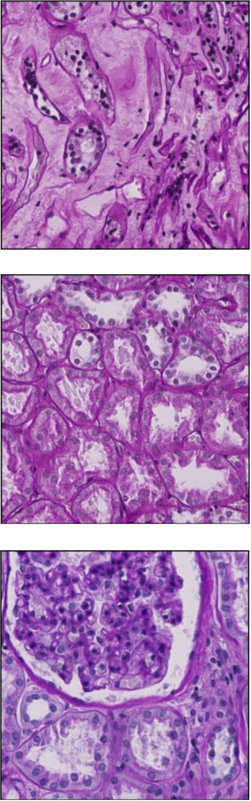
\includegraphics[width=\textwidth]{gambar/bab4/image_hasil.png}
		\caption{Citra test}
		\label{fig:image_hasil}
	\end{subfigure}
	\hfill
	\begin{subfigure}[b]{0.24\textwidth}
		\centering
		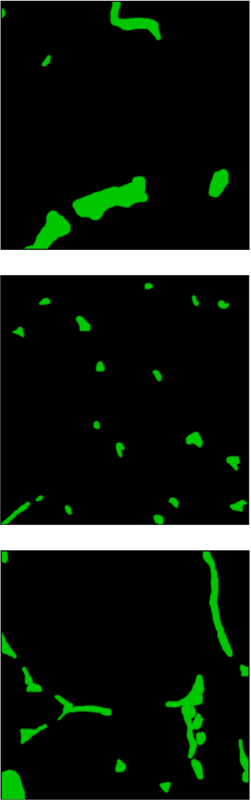
\includegraphics[width=\textwidth]{gambar/bab4/true_label.png}
		\caption{label ground truth}
		\label{fig:true_label}
	\end{subfigure}
	\hfill
	\begin{subfigure}[b]{0.24\textwidth}
		\centering
		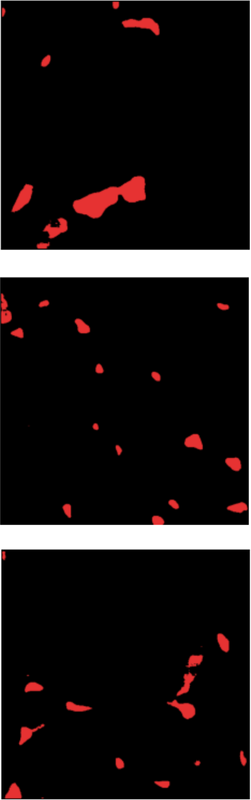
\includegraphics[width=\textwidth]{gambar/bab4/predicted_label.png}
		\caption{Prediksi model}
		\label{fig:predicted_label}
	\end{subfigure}
	\hfill
	\begin{subfigure}[b]{0.24\textwidth}
		\centering
		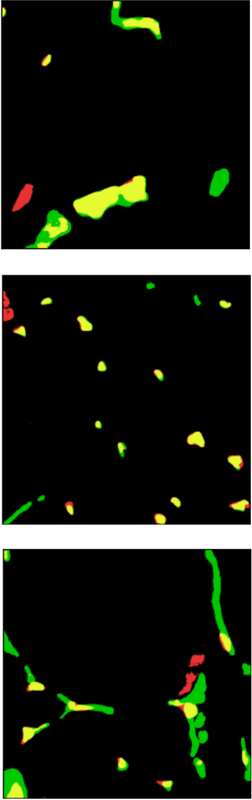
\includegraphics[width=\textwidth]{gambar/bab4/overlayed_label.png}
		\caption{Perbandingan}
		\label{fig:overlayed-label}
	\end{subfigure}
	
	\caption{Sample hasil segmentasi pada data test }
	\label{fig:sample_hasil}
	
\end{figure}

\noindent Gambar \ref{fig:sample_hasil} diatas menyajikan hasil segmentasi pada sample data uji. Untuk membandingkan hasil kita bisa fokus pada panel (d). Area hijau pada panel (d) menunjukkan false negative dimana area yang merupakan pembuluh darah namun tidak diprediksi oleh model. Kemudian area kuning menunjukkan true positive yang merupakan pembuluh darah dan terprediksi oleh model. Sedangkan warna merah mengindikasikan false positive yang merupakan area yang bukan pembuluh darah namun diprediksi model sebagai pembuluh darah.

%\noindent Pada baris pertama, model berhasil memprediksi area yang merupakan pembuluh darah. Meskipun demikian, area yang terprediksi tidak mencakup keseluruhan pembuluh darah area yang seharusnya termasuk pembuluh darah namun masih belum terprediksi oleh model sebagai pembuluh darah. kemudian juga ada sedikit false positive yang bukan pembuluh darah namun diprediksi model sebagai pembulluh darah.

%\noindent Pada baris kedua model berhasil memprediksi sebagian besar pembuluh darah kecil dengan presisi tinggi seperti yang dilihat bewarna kuning pada panel (d). model tampaknya bekerja dengan baik pada pembuluh darah yang berukuran kecil. Namun, terlihat beberapa false positive area merah pada panel (d) di area pinggiran dan juga ada sedikit false negative.

%\noindent pada baris ketiga model tidak bisa benar-benar menangkap bentuk dari pembuluh darah yang diindikasikan oleh warna kuning pada panel (d). Selain itu juga terdapat sedikit false positive pada prediksi model.

\noindent Secara keseluruhan model attention U-net menunjukkan kinerja baik dalam mendeteksi pembuluh darah yang berbentuk bercak-bercak kecil. seperti yang terlihat pada sample pertama sampai ketiga. Tantangan utama dari model ini adalah model tidak mampu menangkap bentuk dari pembuluh darah yang besar yang melibatkan beberapa false negative pada sampel pertama dan ketiga.


\noindent Hasil visualisasi ini menunjukkan bahwa model Attention U-Net memiliki potensi besar dalam mendeteksi mikrovaskular pada WSI jaringan ginjal manusia. Model menunjukkan kekuatan dalam mendeteksi pembuluh darah kecil dengan tingkat recall yang tinggi, seperti terlihat pada panel kedua. Namun, tantangan utama terletak pada segmentasi pembuluh darah besar, yang menghasilkan beberapa false negative seperti pada sampel pertama dan ketiga.





%\begin{table}[H]
%\centering
%\caption{Parameter kelulusan tugas akhir}
%\begin{tabular}{ clc }
%\hline
%\textbf{No.} & \textbf{Parameter } & \textbf{Nilai} \\
%\hline
%1. & Penulisan & A \\
%2. & Penulisan & A \\
%\hline
%\end{tabular}
%\label{table:nilai}
%\end{table}





% Please add the following required packages to your document preamble:
% \usepackage{booktabs}
% \usepackage{multirow}

%Berikut adalah contoh tabel yang dicetak secara horizontal
%gunakan package longtable
%Dapat dibuat dulu di https://www.tablesgenerator.com/ lalu dipindah
%\begin{landscape}
%\begin{longtable}{p{3.5cm}cllllll}
%\caption{Contoh Tabel Mendatar yang Panjang dan Lebar}\\
%\hline
%\textbf{Provinsi} & \textbf{Kode Wilayah} & \textbf{Singkatan Umum} & \textbf{ISO} & \textbf{Pulau} & \textbf{Ibu Kota} & \textbf{Gubernur} \\ \hline
%\endfirsthead

%\multicolumn{4}{l}{\bfseries \tablename\ \thetable{} -- Lanjutan dari halaman sebelumnya}\\
% \begin{center}
% % {{\bfseries \tablename\ \thetable{} -- Lanjutan dari halaman sebelumnya}} \\
% \end{center}
%\hline
%\textbf{Provinsi} & \textbf{Kode Wilayah} & \textbf{Singkatan Umum} & \textbf{ISO} & \textbf{Pulau} & \textbf{Ibu Kota} & \textbf{Gubernur} \\ \hline

%\endhead

%\hline
%\endfoot

%\endlastfoot



%Aceh & 11 & Aceh & ID-AC & Sumatera & Banda Aceh & Achmad Marzuki \\
%Sumatera Utara & 12 & Sumut & ID-SU & Sumatera & Medan & Edy Rahmayadi \\
%Sumatera Barat & 13 & Sumbar & ID-SB & Sumatera & Padang & Mahyeldi Ansharullah \\
%Riau & 14 & Riau & ID-RI & Sumatera & Pekanbaru & Syamsuar \\
%Jambi & 15 & Jambi & ID-JA & Sumatera & Jambi & Al Haris \\
%Sumatera Selatan & 16 & Sumsel & ID-SS & Sumatera & Palembang & Herman Deru \\
%Bengkulu & 17 & Bengkulu & ID-BE & Sumatera & Bengkulu & Rohidin Mersyah \\
%Lampung & 18 & Lampung & ID-LA & Sumatera & Bandar Lampung & Arinal Djunaidi \\
%Kepulauan Bangka Belitung & 19 & Babel & ID-BB & Sumatera & Pangkalpinang & Ridwan Djamaluddin \\
%Kepulauan Riau & 21 & Kepri & ID-KR & Sumatera & Tanjungpinang & Ansar Ahmad \\
%Daerah Khusus Ibukota Jakarta & 31 & DKI Jakarta & ID-JK & Jawa & Tidak ada & Heru Budi Hartono \\
%Jawa Barat & 32 & Jabar & ID-JB & Jawa & Bandung & Ridwan Kamil \\
%Jawa Tengah & 33 & Jateng & ID-JT & Jawa & Semarang & Ganjar Pranowo \\
%Daerah Istimewa Yogyakarta & 34 & DIY & ID-YO & Jawa & Yogyakarta & Hamengkubuwana X \\
%Jawa Timur & 35 & Jatim & ID-JI & Jawa & Surabaya & Khofifah Indar Parawansa \\
%Banten & 36 & Banten & ID-BT & Jawa & Serang & Al Muktabar \\
%Bali & 51 & Bali & ID-BA & Nusa Tenggara & Denpasar & I Wayan Koster \\
%Nusa Tenggara Barat & 52 & NTB & ID-NB & Nusa Tenggara & Mataram & Zulkieflimansyah \\
%Nusa Tenggara Timur & 53 & NTT & ID-NT & Nusa Tenggara & Kupang & Viktor Laiskodat \\

%Kalimantan Barat & 61 & Kalbar & ID-KB & Kalimantan & Pontianak & Sutarmidji \\
%Kalimantan Tengah & 62 & Kalteng & ID-KT & Kalimantan & Palangka Raya & Sugianto Sabran \\
%Kalimantan Selatan & 63 & Kalsel & ID-KS & Kalimantan & Banjarbaru & Sahbirin Noor \\
%Kalimantan Timur & 64 & Kaltim & ID-KI & Kalimantan & Samarinda & Isran Noor \\
%Kalimantan Utara & 65 & Kaltara & ID-KU & Kalimantan & Tanjung Selor & Zainal Arifin Paliwang \\
%Sulawesi Utara & 71 & Sulut & ID-SA & Sulawesi & Manado & Olly Dondokambey \\
%Sulawesi Tengah & 72 & Sulteng & ID-ST & Sulawesi & Palu & Rusdy Mastura \\
%Sulawesi Selatan & 73 & Sulsel & ID-SN & Sulawesi & Makassar & Andi Sudirman Sulaiman \\
%Sulawesi Tenggara & 74 & Sultra & ID-SG & Sulawesi & Kendari & Ali Mazi \\
%Gorontalo & 75 & Gorontalo & ID-GO & Sulawesi & Gorontalo & Hamka Hendra Noer \\
%Sulawesi Barat & 76 & Sulbar & ID-SR & Sulawesi & Mamuju & Akmal Malik \\
%Maluku & 81 & Maluku & ID-MA & Maluku & Ambon & Murad Ismail \\
%Maluku Utara & 82 & Malut & ID-MU & Maluku & Sofifi & Abdul Ghani Kasuba \\
%Papua & 91 & Papua & ID-PA & Papua & Jayapura & Lukas Enembe \\
%Papua Barat & 92 & Pabar & ID-PB & Papua & Manokwari & Paulus Waterpauw \\
%Papua Selatan & 93 & Pasel & — & Papua & Merauke & Apolo Safanpo \\
%Papua Tengah & 94 & Papteng & — & Papua & Nabire & Ribka Haluk \\
%Papua Pegunungan & 95 & Papeg & — & Papua & Wamena & Nikolaus Kondomo \\
%Papua Barat Daya & 96 & PBD & — & Papua & Sorong1 & — \\ \hline
%\label{table:tabelpanjanglebar}
%\end{longtable}
%\end{landscape}


%		\subsection{Subsubbab 2 2}
%		\blindtext

%	\section{Subab 3}
%	\blindtext \ref{fig:komputer}

%\begin{equation}
 %   x+2 = 159
%\end{equation}
%\blindtext

%Berikut adalah contoh gambar yang dicetak secara horizontal
%\begin{landscape}
 %  \begin{figure}[t]
  %      \centering
   %     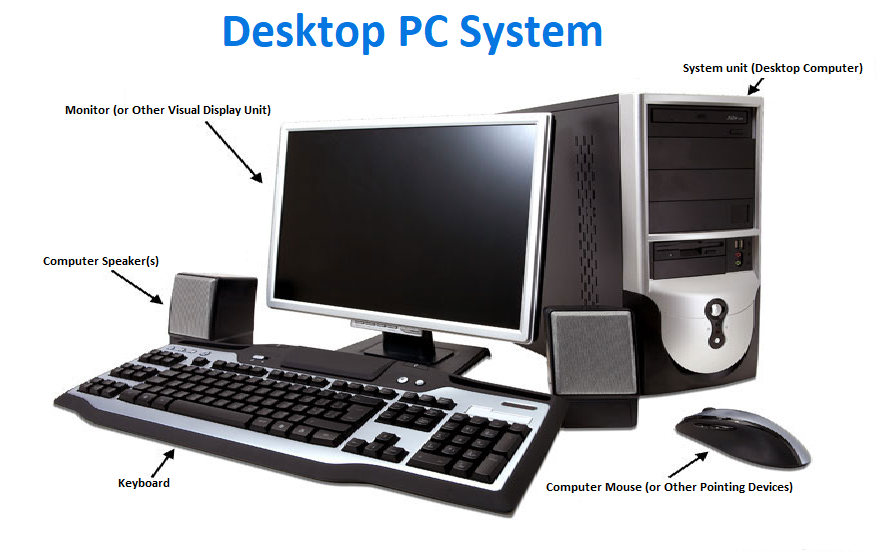
\includegraphics[width=18cm, height=12cm]{gambar/contoh-gambar-miring.png}
    %    \caption{Contoh Gambar Komputer}
     %   \label{fig:komputer}
    %\end{figure}
%\end{landscape}



% Bab 5 penutup
\chapter{KESIMPULAN DAN SARAN}

\section{Kesimpulan}
\noindent Berdasarkan hasil analisis dan pengujian fungsional aplikasi ini, didapat kesimpulan sebagai berikut:

\begin{enumerate}
	\item Lorem ipsum is a pseudo-Latin text used in web design, typography, layout, and printing in place of English to emphasise design elements over content.

	\item It's also called placeholder (or filler) text. It's a convenient tool for mock-ups.

	\item It helps to outline the visual elements of a document or presentation, eg typography, font, or layout. Lorem ipsum is mostly a part of a Latin text by the classical author and philospher Cicero.

	\item Its words and letters have been changed by addition or removal, so to deliberately render its content nonsensical; it's not genuine, correct, or comprehensible Latin anymore.
\end{enumerate}


\section{Saran}
\noindent Hal-hal penting terkait pelaksanaan penelitian yang perlu diperhatikan kedepannya adalah
\begin{enumerate}
	\item Lorem ipsum is a pseudo-Latin text used in web design, typography, layout, and printing in place of English to emphasise design elements over content.

	\item It's also called placeholder (or filler) text. It's a convenient tool for mock-ups.

	\item It helps to outline the visual elements of a document or presentation, eg typography, font, or layout. Lorem ipsum is mostly a part of a Latin text by the classical author and philospher Cicero.

	\item Its words and letters have been changed by addition or removal, so to deliberately render its content nonsensical; it's not genuine, correct, or comprehensible Latin anymore.
\end{enumerate}


% Baris ini digunakan untuk membantu dalam melakukan sitasi
% Karena diapit dengan comment, maka baris ini akan diabaikan
% oleh compiler LaTeX.
\begin{comment}
\bibliography{daftar-pustaka}
\end{comment}


% Daftar Pustaka
\addcontentsline{toc}{chapter}{DAFTAR PUSTAKA}
\sloppy
\printbibliography

% Halaman lampiran di tengah
\newpage
\begin{center}
    \thispagestyle{empty}
    \vspace*{\fill}
    \noindent \Huge{LAMPIRAN}
    \addcontentsline{toc}{chapter}{LAMPIRAN}
\vspace*{\fill}
\end{center}


% Lampiran
\begin{appendix}
\chapter{Perhitungan Aritmatika Pendukung}

\noindent Lampiran ini berisikan contoh perhitungan yang terjadi di dalam model yang dikembangkan dalam penelitian. Perhitungan menggunakan data yang sederhana untuk memberikan pemahaman intuitif terhadap cara kerja model. 

\section{Operasi Konvolusi}
\noindent Pada arsitektur Attention U-net operasi konvolusi menggunakan padding agar output yang dihasilkan tetap memiliki dimensi sama dengan input. Padding adalah penambahan nilai nol di sekitar tepi citra input. Hal ini dilakukan agar setiap piksel pada citra input memberikan kontribusi pada hasil konvolusi sehingga informasi spasial tidak hilang. Berikut adalah gambaran kerja operasi konvolusi dengan tambahan padding disekitar citra input.

\begin{figure}[H]
	\centering
	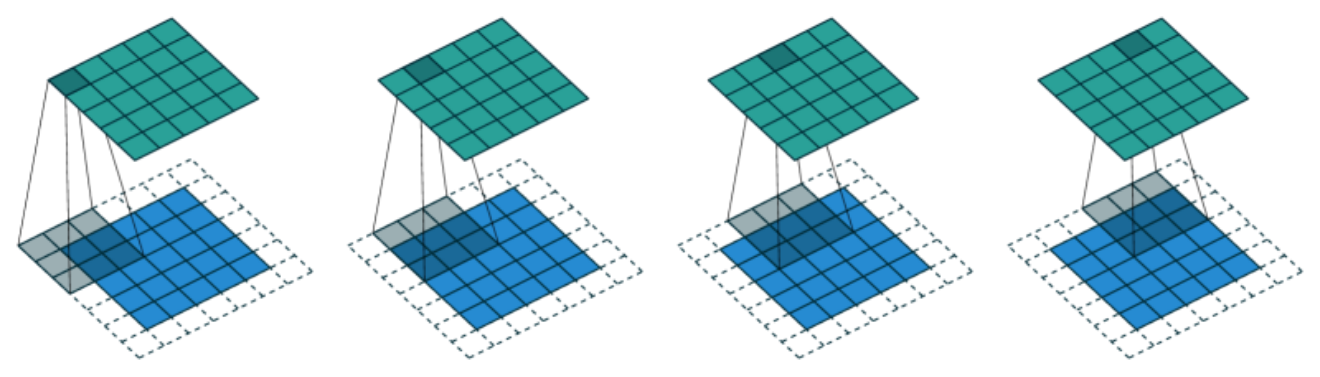
\includegraphics[scale=.4]{gambar/lampiran/stride.png}
\end{figure}

\noindent Selanjutnya contoh perhitungan dari operasi konvolusi menggunakan data yang sederhana:

\begin{figure}[H]
	\centering
	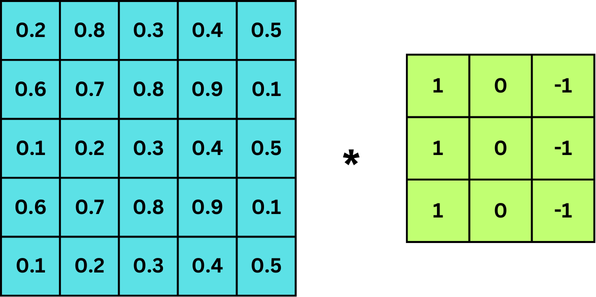
\includegraphics[scale=.3]{gambar/lampiran/konvolusi.png}
\end{figure}

\noindent Anggap kita punya sebuah input citra input 5 x 5 dengan filter edge detection 3 x 3.

\begin{figure}[H]
	\centering
	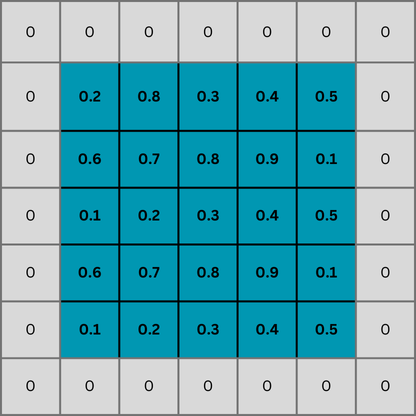
\includegraphics[scale=.3]{gambar/lampiran/padding.png}
\end{figure}

\noindent Langkah pertama adalah penambahan piksel bernilai 0 disekitar citra.


\begin{figure}[H]
	\centering
	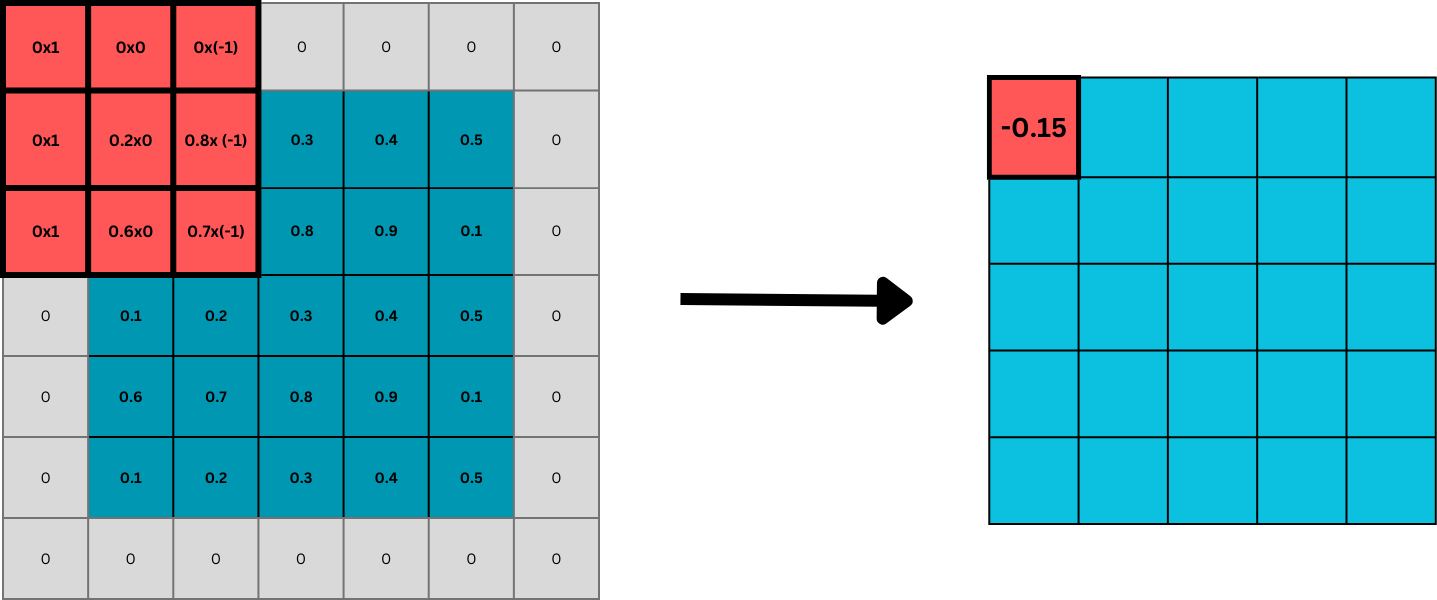
\includegraphics[scale=.3]{gambar/lampiran/posisi-awal.png}
\end{figure}
\noindent Setelah itu filter akan dilakukan perhitungan konvolusi di atas input untuk menghasilkan output di titik \([0,0]\) dengan detail sebagai berikut: 

(1 * 0) + (0 * 0) + (-1 * 0) + (1 * 0) + (0 * 0.2) + (-1 * 0.8) + (1 * 0) + (0 * 0.6) + (-1 * 0.7) = -1.5


\begin{figure}[H]
	\centering
	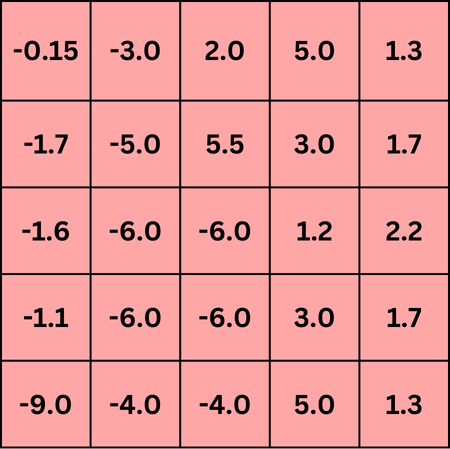
\includegraphics[scale=.3]{gambar/lampiran/hasil-konvolusi.png}
\end{figure}

\noindent Setelah semua bagian input dilakukan perhitungan konvolusi, akan menghasilkan output seperti di atas.

\section{Pooling}


\noindent Operasi pooling yang digunakan pada attention U-net adalah max-pooling. Max-pooling mengambil nilai maksimum dari setiap wilayah yang dilewati oleh filter.  Ukuran filter yang umum digunakan adalah 2x2, dengan stride (langkah) sebesar 2.  Artinya, filter akan bergerak 2 langkah secara horizontal dan vertikal pada setiap iterasi. berikut adalah contoh dari penerapan max-pooling pada input sederhana 4 x 4 dan filter yang digunakan 2 x 2.

\begin{figure}[H]
	\centering
	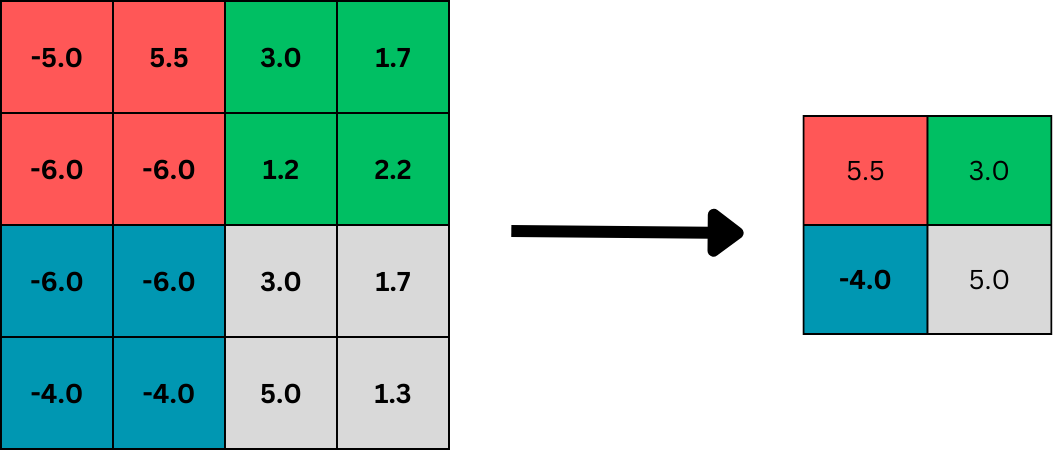
\includegraphics[scale=.3]{gambar/lampiran/pooling.png}
\end{figure}

\noindent Pada contoh diatas daerah yang dilewati filter 2 x 2 diambil nilai paling tinggi untuk menjadi nilai pada output.

\section{Transpose Konvolusi}

\noindent Transpose konvolusi menggunakan filter untuk menghasilkan peningkatan resolusi peta fitur hasil \textit{down-sampling}. Pada Attention U-net filter transpose konvolusi diterapkan pada output dengan stride 2. Contoh penerapan pada data sederhana adalah sebagai berikut:

\begin{figure}[H]
	\centering
	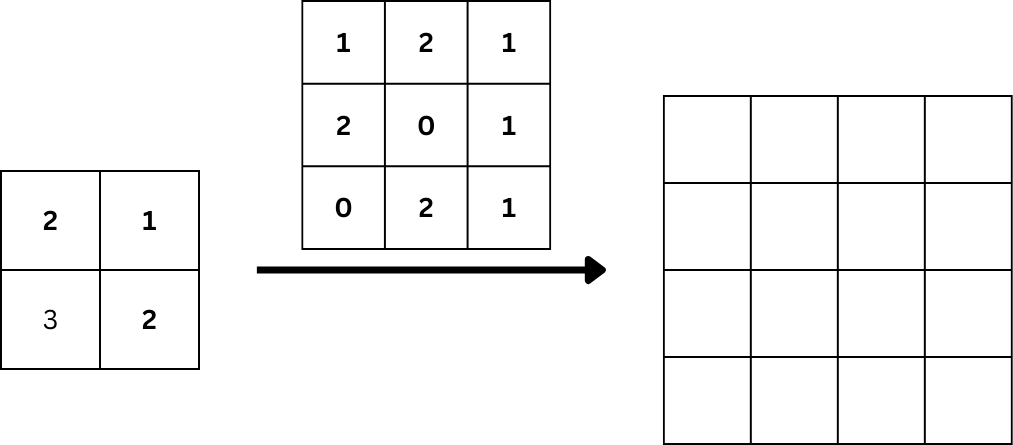
\includegraphics[scale=.3]{gambar/lampiran/dekonv-1.png}
\end{figure}

\noindent Anggap kita punya peta fitur 2 x 2 yang akan ditingkatkan resolusinya menjadi 4 x 4 dengan filter 3 x 3.

\begin{figure}[H]
	\centering
	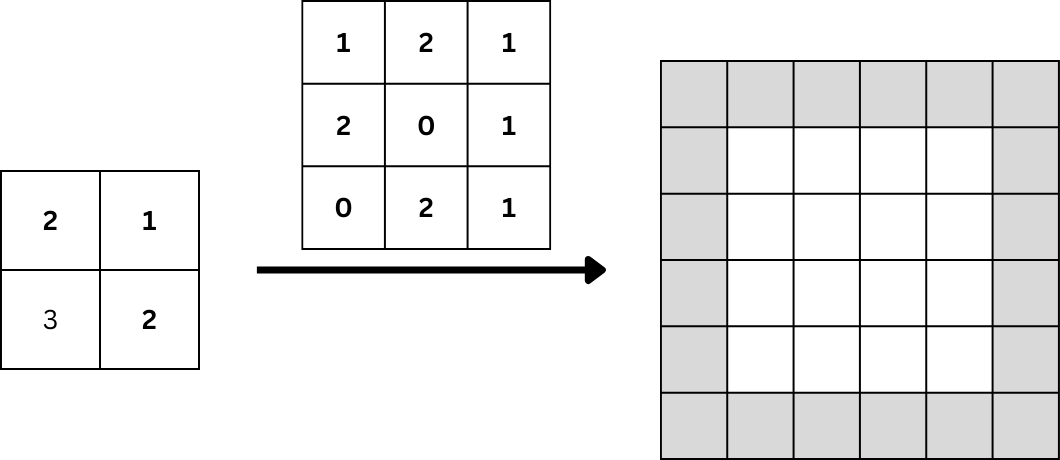
\includegraphics[scale=.3]{gambar/lampiran/dekonv-2.png}
\end{figure}

\noindent Langkah pertama adalah penambahan padding disekitar output agar operasi konvolusi bisa dilakukan.

\begin{figure}[H]
	\centering
	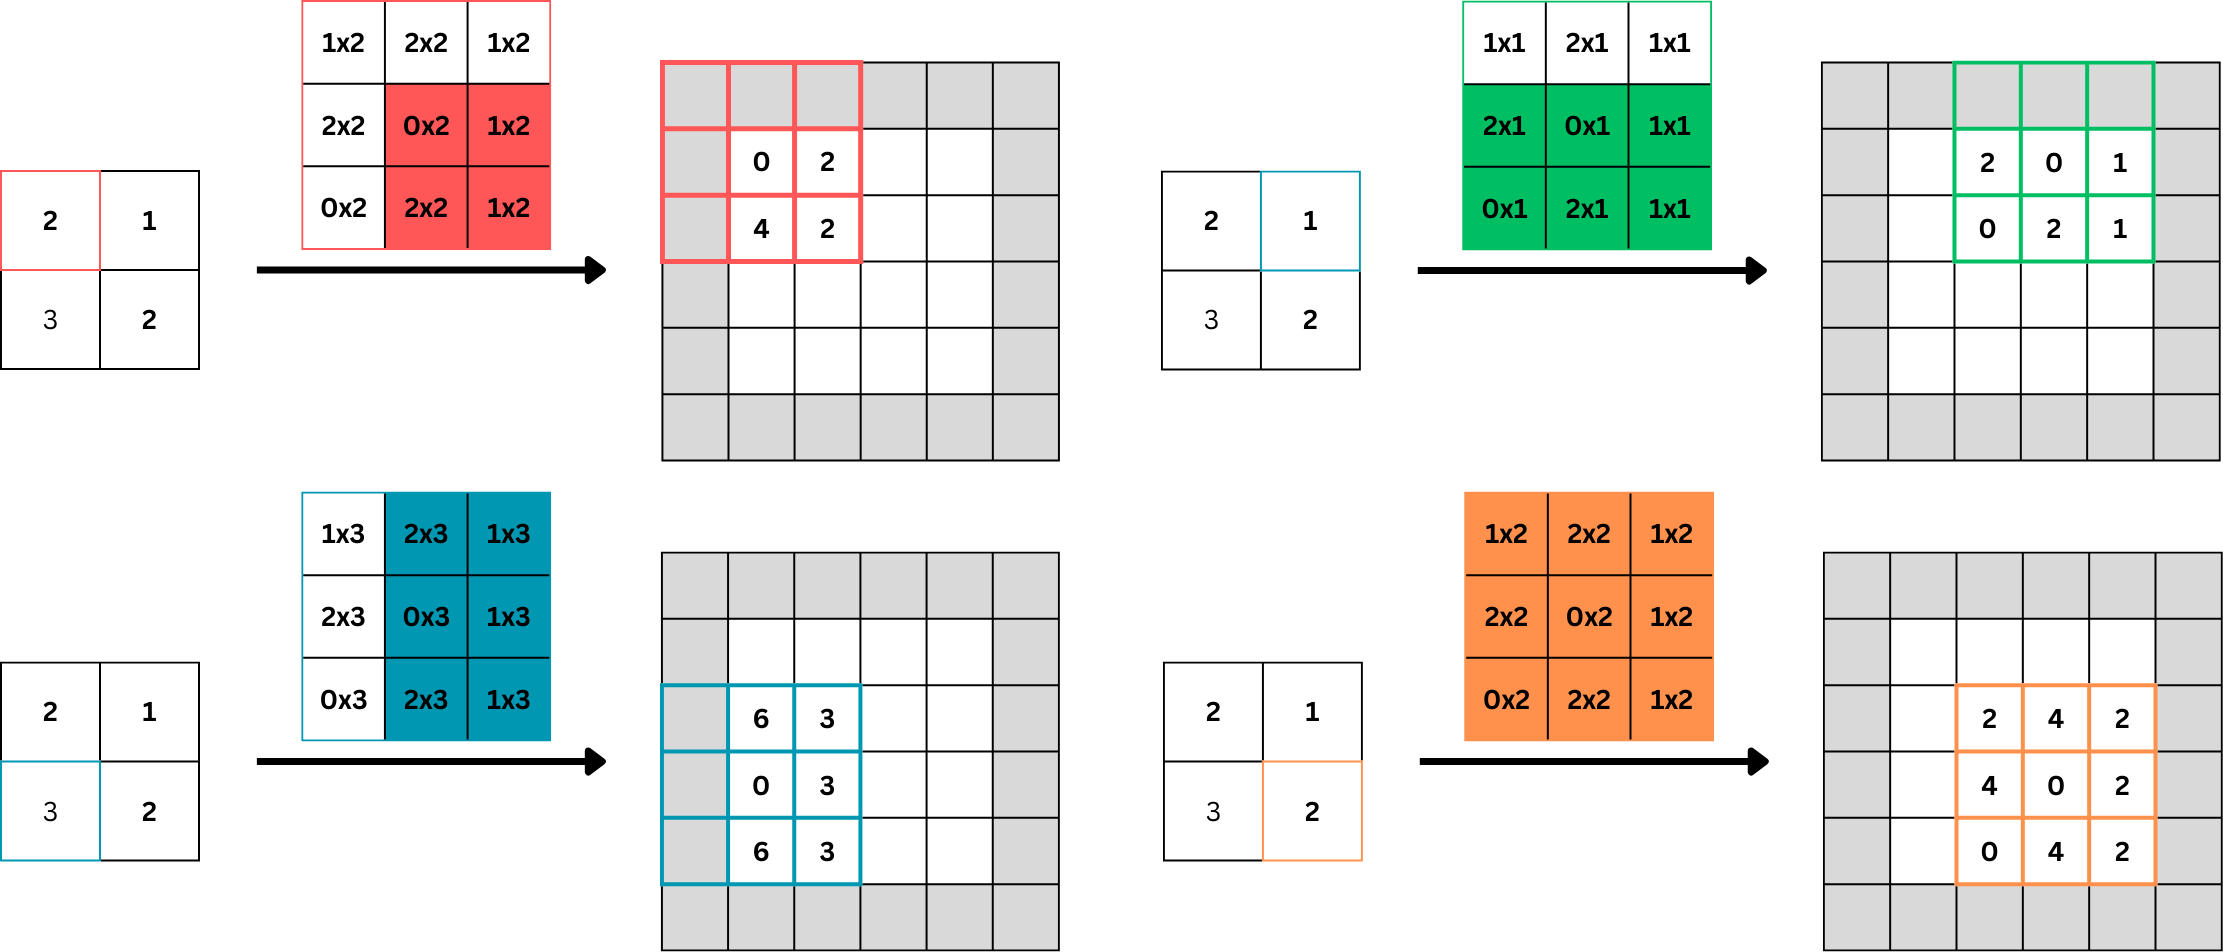
\includegraphics[scale=.2]{gambar/lampiran/dekonv-full.png}
\end{figure}

Selanjutnya input akan diambil dan dikalikan dengan setiap nilai yang ada pada filter. Area padding dihiraukan.

\begin{figure}[H]
	\centering
	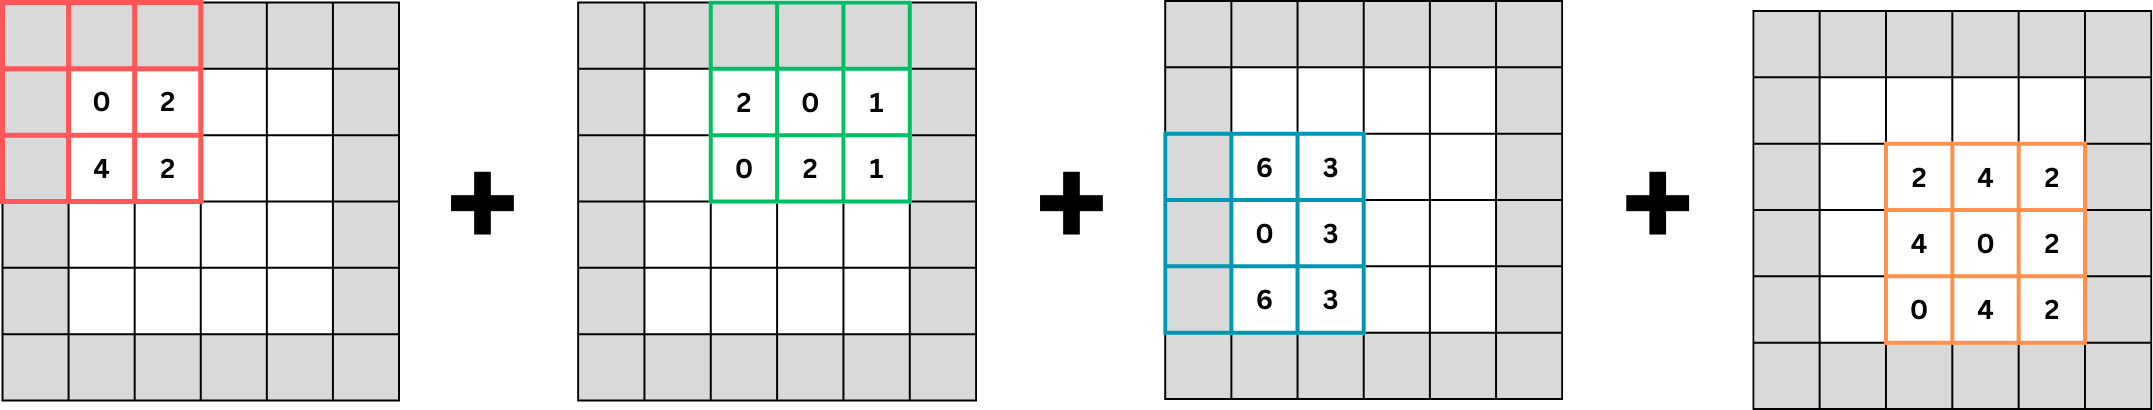
\includegraphics[scale=.2]{gambar/lampiran/dekonv-7.png}
\end{figure}

Kemudian hasil perkalian yang ada pada setiap area output akan dijumlahkan.

\begin{figure}[H]
	\centering
	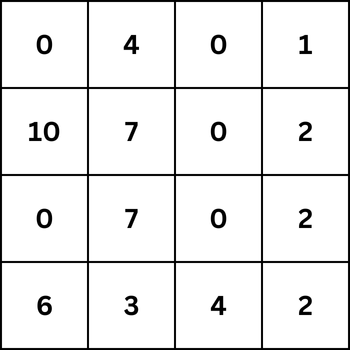
\includegraphics[scale=.3]{gambar/lampiran/dekonv-8.png}
\end{figure}

%Terakhir are padding dihilangkan sehingga kita mendapatkan output 4 x 4 seperti yang diinginkan.

\section{Fungsi Aktivasi}

\begin{figure}[H]
	\centering
	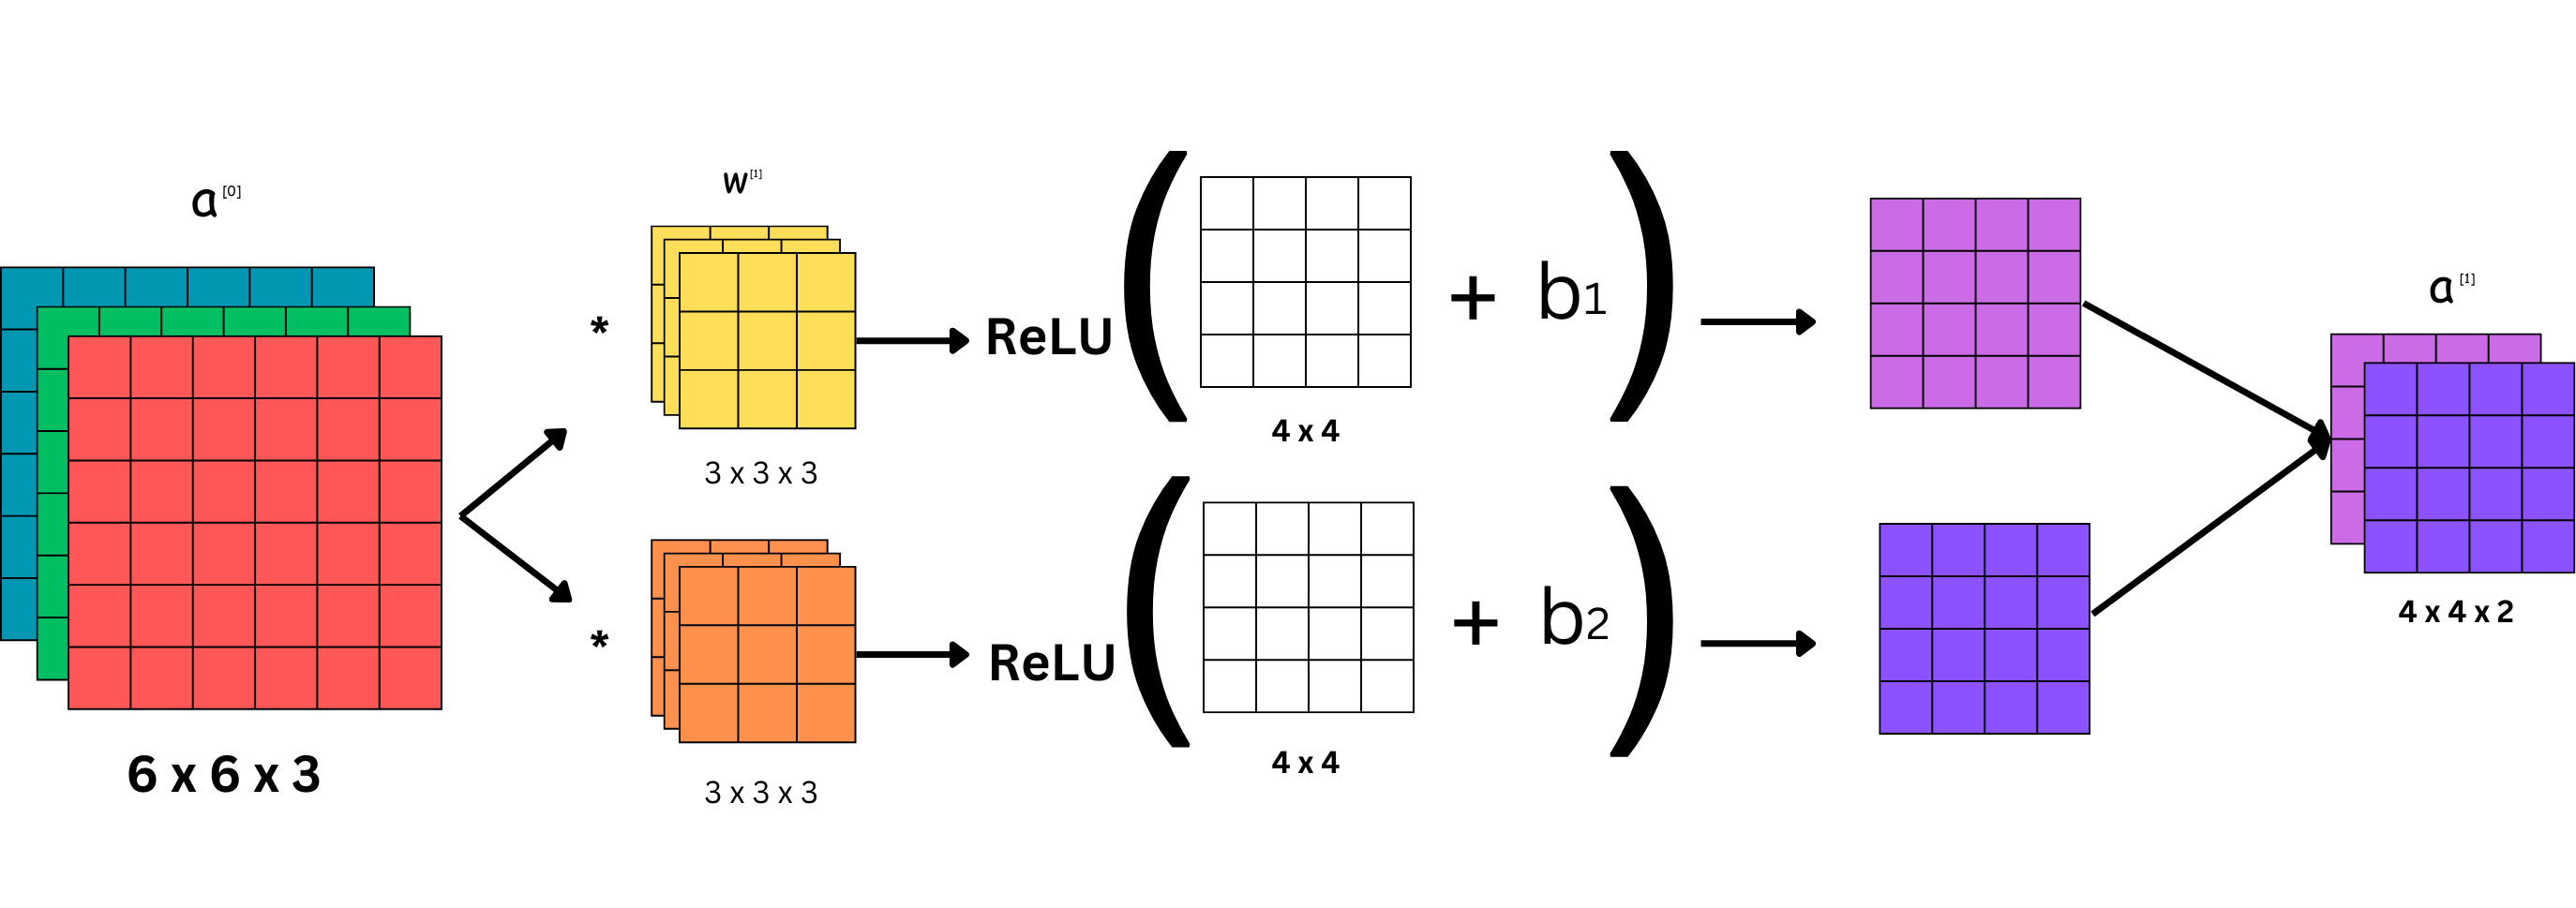
\includegraphics[scale=.2]{gambar/lampiran/feed-fwrd.png}
\end{figure}

\noindent Gambar diatas merupakan contoh sebuah layer konvolusi. Setelah dihasilkan peta fitur, jaringan akan menambahkan bias pada peta fitur tersebut untuk mengatur nilai output dari neuron. Kemudian, fungsi aktivasi ReLU (Rectified Linear Unit) diterapkan pada setiap elemen feature map. ReLU mengubah semua nilai negatif menjadi nol, dan mempertahankan nilai positif apa adanya. Berikut adalah contoh dari penerapan ReLU pada peta fitur.

\begin{figure}[H]
	\centering
	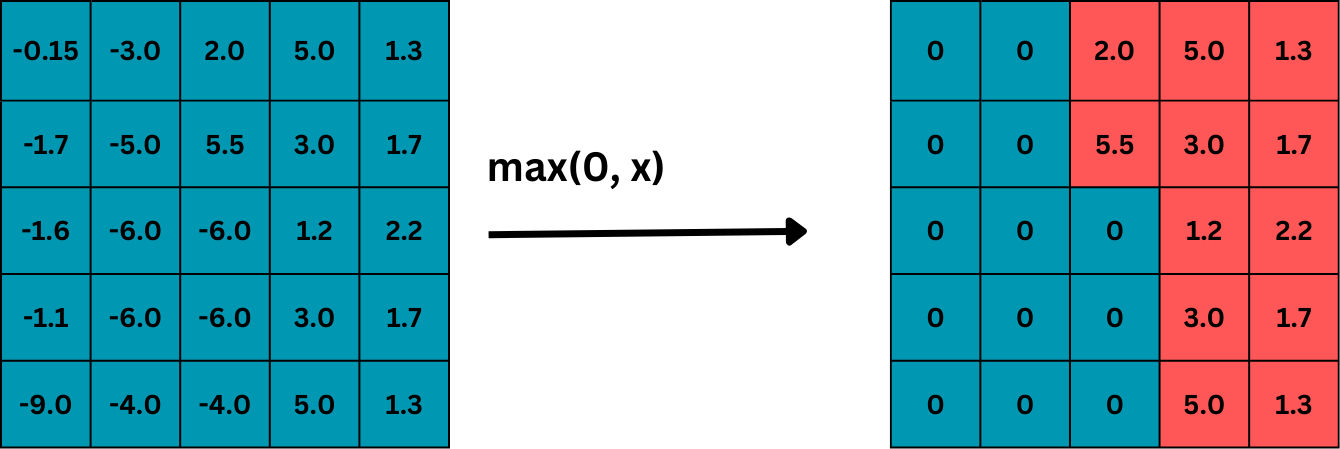
\includegraphics[scale=.2]{gambar/lampiran/fungsi-relu.png}
\end{figure}

ReLU mengubah setiap nilai negatif menjadi 0 dan mempertahankan nilai positif apa adanya. Sebagai contoh, untuk elemen pertama (-0.15), karena nilainya negatif, maka ReLU(-0.15) = 0.  Untuk elemen ketiga (2.0), karena nilainya positif, maka ReLU(2.0) = 2.0.

\noindent Fungsi aktivasi sigmoid memiliki cara kerja yang sama dengan ReLu, dimana fungsi ini akan diterapkan pada setiap elemen dari peta fitur. berikut adalah contoh perhitungan dari fungsi aktivasi sigmoid pada peta fitur yang sama dengan perhitungan pada contoh ReLU:

\[
\sigma(-0.15) = \frac{1}{1 + e^{0.15}} \approx 0.46257
\]

\[
\sigma(-3.0) = \frac{1}{1 + e^{3.0}} \approx 0.04743
\]

\[
\sigma(2.0) = \frac{1}{1 + e^{-2.0}} \approx 0.88080
\]

\[
\sigma(5.0) = \frac{1}{1 + e^{-5.0}} \approx 0.99331
\]

\[
\sigma(1.3) = \frac{1}{1 + e^{-1.3}} \approx 0.78583
\]



\section{Evaluasi}
 
 \noindent Pada Attention U-net, evaluasi yang digunakan untuk melihat kemampuan model dalam memprediksi objek adalah Interseption ove Union (IoU) dan Dice Similarity Coefficient (DSC). Beirikut ini adalah contoh perhitungan evaluasi model.
 
 \begin{figure}[H]
 	\centering
 	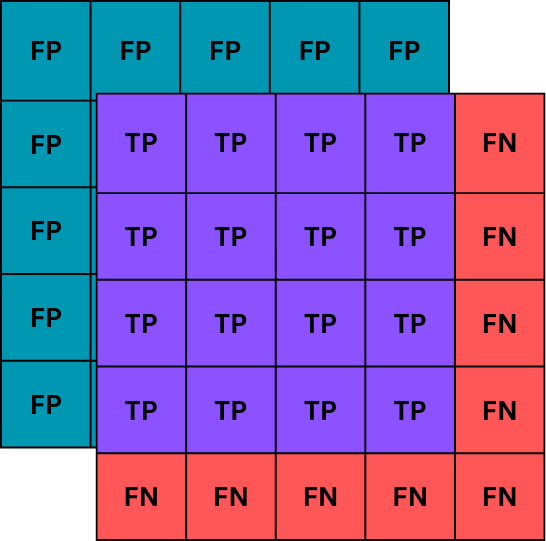
\includegraphics[scale=.2]{gambar/lampiran/prediksi.png}
 \end{figure}    
 
 \noindent Anggap kita punya kotak biru (ground truth) yang mewakili objek sebenarnya dan kotak merah (prediksi) yang merupakan prediksi model tentang lokasi dan ukuran objek. True positive (TP) merupakan area tumpang tindih antara kotak biru dan kotak merah, merupakan prediksi benar. False positive (FP) area kotak merah yang tidak tumpang tindih dengan kotak biru, merupakan prediksi yang salah. False negative (FN) area kotak biru yang tidak tumpang tindih dengan kotak merah, merupakan area objek yang tidak terdeteksi model.    
 
  \begin{figure}[H]
 	\centering
 	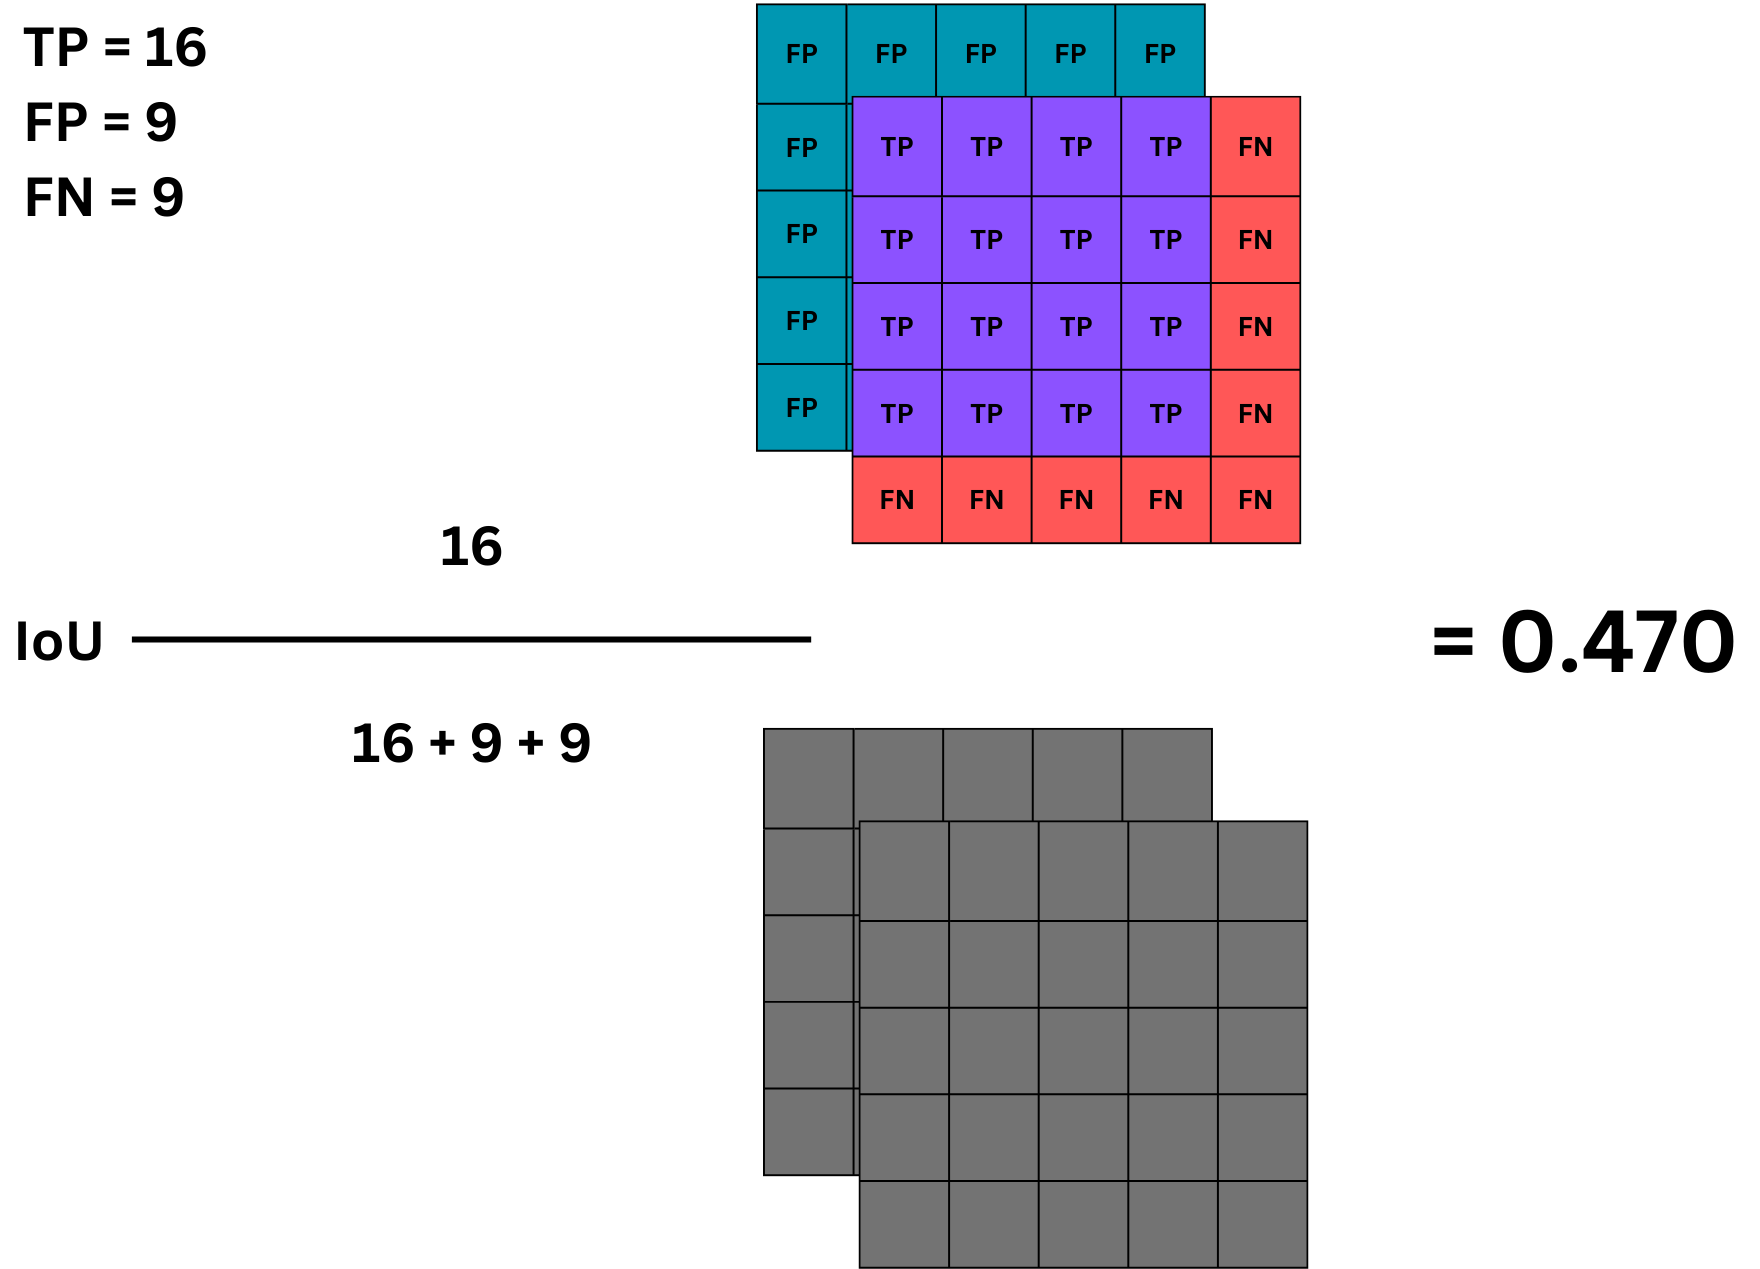
\includegraphics[scale=.2]{gambar/lampiran/IoU.png}
 \end{figure} 
 
 IoU dihitung dengan membagi luas area tumpang tindih (TP) dengan luas gabungan dari kedua kotak (TP + FP + FN). Begitu juga dengan DSC membagi dua kali area tumpang tindih (2TP) dengan luas gabungan (2TP + FP FN). 
 

\section{Sample Gambar dari Setiap Sumber Whole Slide Image}
\label{sec:sample_gambar}

Pada sub-lampiran ini di tampilkan beberapa sampel citra dari setiap sumber WSI untuk melihat bagaimana karakteristik citra di setiap WSI.

\begin{figure}[H]
	%\begin{subfigure}[b]{1\textwidth}
	\centering
	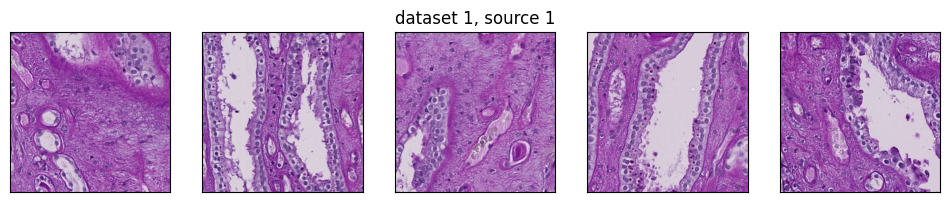
\includegraphics[width=\textwidth]{gambar/bab4/ds1s1_0.png}
	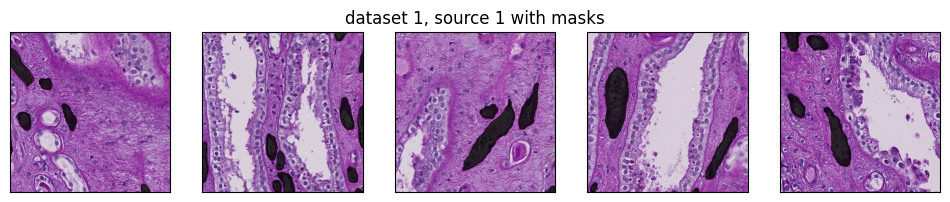
\includegraphics[width=\textwidth]{gambar/bab4/ds1s1_1.png}
	
\includegraphics[width=\textwidth]{gambar/bab4/ds1s1_2.png}
	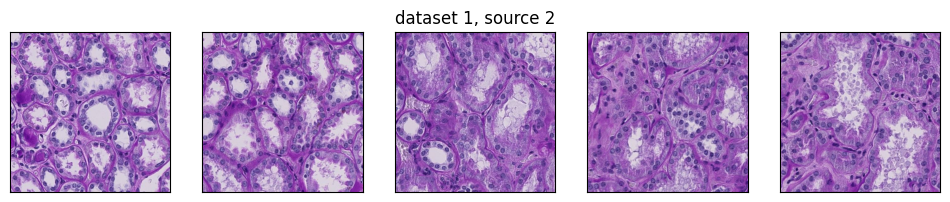
\includegraphics[width=\textwidth]{gambar/bab4/ds1s2_0.png}
	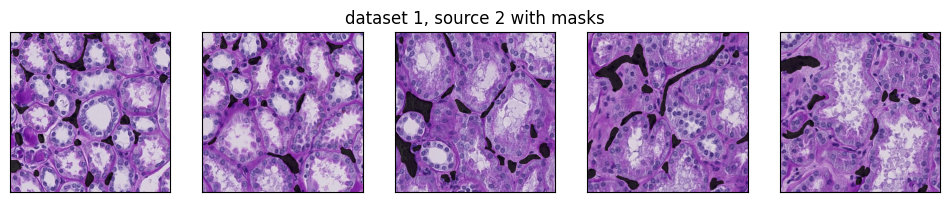
\includegraphics[width=\textwidth]{gambar/bab4/ds1s2_1.png}
	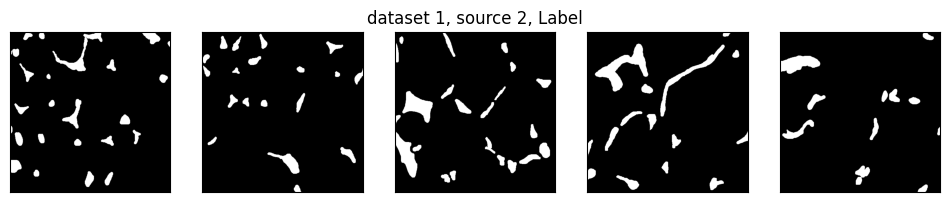
\includegraphics[width=\textwidth]{gambar/bab4/ds1s2_2.png}
	%\caption{Sample citra pada dataset 1}
	\label{fig:ds1_image}
	%\end{subfigure}	
	
\end{figure}


\begin{longtable}{c}
	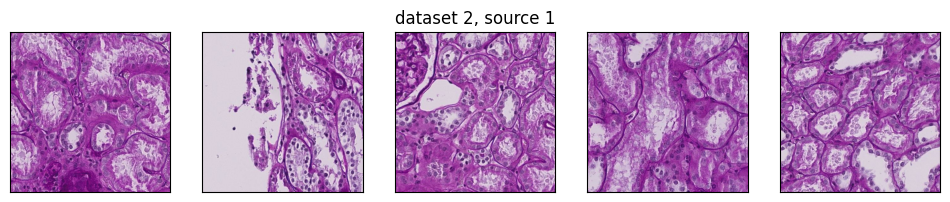
\includegraphics[width=\textwidth]{gambar/bab4/ds2s1_0.png} \\
	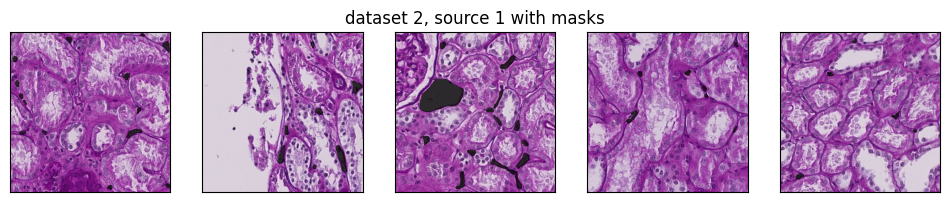
\includegraphics[width=\textwidth]{gambar/bab4/ds2s1_1.png} \\
	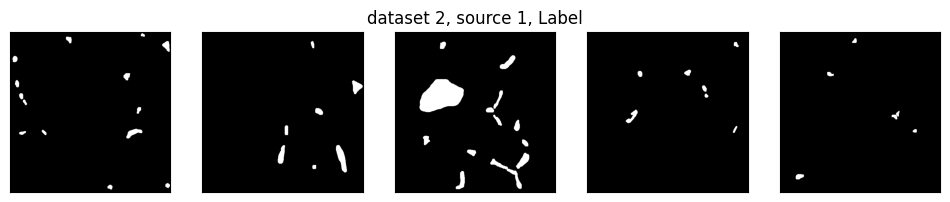
\includegraphics[width=\textwidth]{gambar/bab4/ds2s1_2.png} \\
	
	
	\includegraphics[width=\textwidth]{gambar/bab4/ds2s2_0.png} \\
	\includegraphics[width=\textwidth]{gambar/bab4/ds2s2_1.png} \\
	\includegraphics[width=\textwidth]{gambar/bab4/ds2s2_2.png} \\
	
	\includegraphics[width=\textwidth]{gambar/bab4/ds2s3_0.png} \\
	\includegraphics[width=\textwidth]{gambar/bab4/ds2s3_1.png} \\
	\includegraphics[width=\textwidth]{gambar/bab4/ds2s3_2.png} \\
	
	\includegraphics[width=\textwidth]{gambar/bab4/ds2s4_0.png} \\
	\includegraphics[width=\textwidth]{gambar/bab4/ds2s4_1.png} \\
	\includegraphics[width=\textwidth]{gambar/bab4/ds2s4_2.png} \\
	
	
\end{longtable}

%\chapter{Hasil Pengamatan} \label{lampiranD}
%\noindent Lampiran hasil pengamatan berisikan dengan \textit{logbook} selama pengamatan, citra objek, keluaran algoritma, skrip pengolahan data dengan Python, dan dokumentasi selama pengamatan.
    %\section{\textit{Logbook} Pengamatan}
     %\noindent Lorem ipsum dolor sit amet, consectetur adipiscing elit, sed do eiusmod tempor incididunt ut labore et dolore magna aliqua. Ut enim ad minim veniam, quis nostrud exercitation ullamco laboris nisi ut aliquip ex ea commodo consequat. Duis aute irure dolor in reprehenderit in voluptate velit esse cillum dolore eu fugiat nulla pariatur. Excepteur sint occaecat cupidatat non proident, sunt in culpa qui officia deserunt mollit anim id est laborum.
    %\section{Objek pada Citra Pengamatan}
    %\noindent Lorem ipsum dolor sit amet, consectetur adipiscing elit, sed do eiusmod tempor incididunt ut labore et dolore magna aliqua. Ut enim ad minim veniam, quis nostrud exercitation ullamco laboris nisi ut aliquip ex ea commodo consequat. Duis aute irure dolor in reprehenderit in voluptate velit esse cillum dolore eu fugiat nulla pariatur. Excepteur sint occaecat cupidatat non proident, sunt in culpa qui officia deserunt mollit anim id est laborum

    %\section{Dokumentasi Pengamatan}
  %\noindent Lorem ipsum dolor sit amet, consectetur adipiscing elit, sed do eiusmod tempor incididunt ut labore et dolore magna aliqua. Ut enim ad minim veniam, quis nostrud exercitation ullamco laboris nisi ut aliquip ex ea commodo consequat. Duis aute irure dolor in reprehenderit in voluptate velit esse cillum dolore eu fugiat nulla pariatur. Excepteur sint occaecat cupidatat non proident, sunt in culpa qui officia deserunt mollit anim id est laborum

%\chapter{Program} \label{lam:lampiran_a}
%\begin{lstlisting}[language=Python]
%import numpy as np

%def incmatrix(genl1,genl2):
 %   m = len(genl1)
  %  n = len(genl2)
   % M = None #to become the incidence matrix
    %VT = np.zeros((n*m,1), int)  #dummy variable

    %#compute the bitwise xor matrix
    %M1 = bitxormatrix(genl1)
 %   M2 = np.triu(bitxormatrix(genl2),1)

  %  for i in range(m-1):
   %     for j in range(i+1, m):
    %        [r,c] = np.where(M2 == M1[i,j])
     %       for k in range(len(r)):
      %          VT[(i)*n + r[k]] = 1;
       %         VT[(i)*n + c[k]] = 1;
        %        VT[(j)*n + r[k]] = 1;
         %       VT[(j)*n + c[k]] = 1;

          %      if M is None:
           %         M = np.copy(VT)
            %    else:
             %       M = np.concatenate((M, VT), 1)

              %  VT = np.zeros((n*m,1), int)

  %  return M
%\end{lstlisting}

%\chapter{Grafik Tambahan} \label{lampiran B}
 %\noindent Lorem ipsum dolor sit amet, consectetur adipiscing elit, sed do eiusmod tempor incididunt ut labore et dolore magna aliqua. Ut enim ad minim veniam, quis nostrud exercitation ullamco laboris nisi ut aliquip ex ea commodo consequat. Duis aute irure dolor in reprehenderit in voluptate velit esse cillum dolore eu fugiat nulla pariatur. Excepteur sint occaecat cupidatat non proident, sunt in culpa qui officia deserunt mollit anim id est laborum

\end{appendix}

\end{document}
